\chapter{Approximation algorithm for phasing}



% \begin{abstract}
    We consider the problem Minimum Error Correction (\MEC).
    A MEC instance is an $n \times m$ matrix $M$ with entries from $\{0,1,-\}$. 
    Feasible solutions are composed of two binary $m$-bit strings, together with an assignment of each row of $M$ to one of the two strings.
    The objective is to minimize the number of mismatches (errors) where the row has a value that differs from the assigned solution string.
    The symbol ``$-$'' is a wildcard that matches both $0$ and $1$.
    A \MEC instance is gapless, if in each row of $M$ all binary entries are consecutive.

    \GMEC is a relevant problem in computational biology, and it is closely related to segmentation problems that were introduced by {[}Kleinberg--Papadimitriou--Raghavan STOC'98{]} in the context of data mining.

    Without restrictions, it is known to be $\UG$-hard to compute an $O(1)$-approximate solution to \MEC. For both \MEC and \GMEC, the best polynomial time approximation algorithm has a logarithmic performance guarantee.
    We partially settle the approximation status of \GMEC by providing a quasi-polynomial time approximation scheme (QPTAS).
    Additionally, for the relevant case where the binary part of a row is not contained in the binary part of another row, we provide a polynomial time approximation scheme (PTAS).
% \end{abstract}
\thispagestyle{empty}

\newpage{}

\setcounter{page}{1}

\section{Introduction.}
The minimum error correction problem (\MEC) is a segmentation problem where we have to partition a set of length $m$ strings into two classes.
A \MEC instance is given by a set of $n$ strings over $\{0,1,-\}$ of length $m$, where the symbol ``$-$'' is a wildcard symbol.
The strings are represented by an $n \times m$ matrix $M$, where the $i$th string determines the $i$th row $M_{i,*}$ of $M$.

The distance $\dist$ of two symbols $a,a'$ from $\{0,1,-\}$ is
\[
    \dist(a,a') := \left\{
        \begin{array}{ll}
            1\colon & a=0,a'=1 \mbox{ or } a=1, a'=0\\ 
            0\colon & \mbox{otherwise.}
        \end{array}
    \right.
\]
For two strings $s,s'$ from $\{0,1,-\}^m$ where $s_j, s'_j$ denotes the $j$-th symbol of the respective string, $\dist(s,s') := \sum_{j=1}^m \dist(s_j,s'_j)$.
A feasible solution to the \MEC is a pair of two strings $\sigma,\sigma'$ from $\{0,1\}^m$.
The optimization goal is to find a feasible solution $(\sigma,\sigma')$ that minimizes
\[
    \cost(\sigma,\sigma') := \sum_{i=1}^{n} \min\{\dist(M_{i,*},\sigma), \dist(M_{i,*},\sigma')\}\,.
\]

A \MEC instance is called \emph{gapless} if in each of the $n$ rows of $M$, all entries from $\{0,1\}$ are consecutive. 
(As regular expression, a valid row is a word of length $m$ from the language $-^*\{0,1\}^*-^*$).
The \MEC problem restricted to gapless instances is \GMEC.

Our motivation to study \GMEC stems from its applications in computational biology.
Humans are diploid, and hence there exist two versions of each chromosome.
% one inherited from the mother and the other from the father. 
Determining the DNA sequences of these two chromosomal copies -- called haplotypes -- is important for many applications ranging from population history to clinical questions~\cite{snyder2015haplotype, tewhey2011importance}. 
Many important biological phenomena such as compound heterozygosity, allele-specific events like DNA methylation or gene expression can only be studied when haplotype-resolved genomes are available~\cite{leung2015integrative}. 

Existing sequencing technologies cannot read a chromosome from start to end, but instead deliver small pieces of the sequences (called reads). 
Like in a jigsaw puzzle, the underlying genome sequences are reconstructed from the reads by finding the overlaps between them.
%Humans and many other organisms are diploids and hence, there are two genome sequences called haplotypes that represent an individual.

The upcoming next-generation sequencing technologies (e.g., Pacific Biosciences) have made the production of relatively long continuous sequences with sequencing errors feasible, where the sequences come from both copies of chromosome.
%The upcoming next-generation sequencing technologies (Pacific Biosciences and Oxford Nanopore Technologies) are used to read these genomes, but they cannot produce reads of entire haplotypes.
%These sequences are aligned to the reference genome or contigs from overlap graph and representing these aligned sequences in the form of Gapless-MEC is straightforward. 
These sequences are aligned to a reference genome or to a structure called contig. 
%As result we one obtains an overlap graph and representing these aligned sequences in the form of Gapless-MEC is straightforward. 
We can formulate the result of this process as a \GMEC instance.
%Haplotyping has several applications including the development of personalized medicine and the study of human migration, evolutionary selection, and population structure~\cite{GCR14_whole}.
%The importance of gapless instances for haplotyping problems was discussed by Lancia et al.~\cite{LBI+01_snps}.

We can therefore formulate haplotyping as the problem of reconstructing the genomes from sequences represented in the form of \GMEC instances by correcting the sequencing errors.
The use of sequencing datasets for complete haplotype phasing is quickly becoming reality~\cite{chin2016phased, chaisson2015resolving}.

%In Computational Biology, some organisms are diploids and hence, there are two genome sequences called haplotypes that represent an individual.
%The upcoming next-generation sequencing (NGS) technologies (Pacific Biosciences) has made the production of longer continuous erroneous sequences feasible, where the sequences come from both the copies of chromosome.
%These sequences are aligned to the reference genome or contigs from overlap graph and representing these aligned sequences in the form of Gapless-MEC is straightforward. 
%The haplotyping addresses the problem of reconstructing the genomes from sequences represented in the form of Gapless-MEC by correcting the sequencing errors.
%Therefore, the use of sequencing data-sets for complete haplotype phasing is fast becoming a reality~\cite{snyder2015haplotype, chin2016phased, tewhey2011importance, chaisson2015resolving}.
%Many important biological

\GMEC is a generalization of a problem called \BMEC, the version of \MEC with only instances $M$ where all entries of $M$ are in $\{0,1\}$.
Finding an optimal solution to \BMEC is equivalent to solving the hypercube 2-segmentation problem (H2S) which was introduced by Kleinberg, Papadimitriou, and Raghavan~\cite{KPR98_segmentation,KPR04_segmentation} and which is known to be $\NP$-hard \cite{Fei14_np,KPR04_segmentation}.
%In particular, the $\NP$-hardness of H2S directly implies the $\NP$-hardness of \BMEC, \GMEC, and \MEC.
The optimization version of \BMEC  differs from H2S in that we minimize the number of mismatches instead of maximizing the number of matches.
\BMEC allows for good approximations.
Ostravsky and Rabiny~\cite{OR02_polynomial} obtained a PTAS for \BMEC based on random embeddings.
Building on the work of Li et al.~\cite{LMW02_finding}, Jiao et al.~\cite{JXL04_k} presented a deterministic PTAS for \BMEC.

\GMEC was shown to be $\NP$-hard by Cilibrasi et al.~\cite{CIKT07_complexity}.\footnote{Their result predates the hardness result of Feige~\cite{Fei14_np} for H2S. The proof of the claimed $\NP$-hardness of H2S by Kleinberg, Papadimitriou, and Raghavan~\cite{KPR98_segmentation} was never published.}
Additionally, they showed that allowing a single gap in each strings renders the problem $\APX$-hard.
More recently, Bonizzoni et al.~\cite{BDK+16_minimum} showed that it is unique games hard to approximate \MEC with constant performance guarantee, whereas it is approximable within a logarithmic factor in the size of the input. 
To our knowledge, previous to our result their logarithmic factor approximation was also the best known approximation algorithm for \GMEC.

\subsection{Our results.}
We provide a quasi-polynomial time approximation scheme (QPTAS) for \GMEC and thus partially settle the approximability for this problem: \GMEC is not $\APX$-hard unless $\NP \subseteq \QP$ (cf.~\cite{RS09_approximation}).
Thus our result reveals a separation of the hardness of the gapless case and the case where we allow a single gap.
Furthermore, already \BMEC is strongly $\NP$-hard since the input does not contain numerical values. 
Therefore we can exclude the existence of an FPTAS for both $\BMEC$ and $\GMEC$ unless $\P = \NP$.

Furthermore, we address the class of \emph{subinterval-free} \GMEC instances where no string is contained in another string.
More precisely, for each pair of rows from $M$ we exclude that the set columns with binary entries from one row is a strict subset of
the set of columns with binary entries from the other row.
We provide a PTAS for subinterval-free instances.

\subsection{Overview of our approach.}

Our algorithm is a dynamic program (DP) that is composed of several levels.
Given a general \GMEC instance, we decompose the rows of the instance into length classes according to the length of the continuous binary parts of the rows.
For each length class we consider a well-selected set of columns such that each row crosses at least one the columns and at most two.
(We say that a row crosses a column if the binary part of the row contains that column.)

We further decompose each length class into two sub-classes, one that crosses exactly one column and one that crosses exactly two columns.
For the second class, it is sufficient to consider every other column, which leaves us with many \emph{rooted} instances.
Thus for each sub-instance there is a single column (the root) which is crossed by all rows of the instance.

We further decompose rooted sub-instances into the left hand side and the right hand side of the root.
We can arrange the rows and columns of these instances in such a way that all rows cross the first column.
We order the rows from top to bottom by increasing length.

The first level of our DP solves these highly structured instances.
The basic idea that we want to apply is that we want to select a constant number of rows from the instance that represents the solution.
This strategy fails because of differing densities within the instance: the selected rows have to represent both the entries of columns crossed by many short rows and entries of arbitrarily small numbers of rows crossing many columns.
To resolve this issue, we observe that computing the solution strings $\sigma$ and $\sigma'$ is equivalent to finding a partition of $M$ into two row sets, one assigned to $\sigma$ and the other assigned to $\sigma'$.
If we assume to have the guarantee that for both solution strings $\sigma$ and $\sigma'$ an $\epsilon$ fraction of rows of the matrix $M$ forms a \BMEC sub-instance, we show that the idea above works.

This insight motivates to separate the instance from left to right into sub-problems with the required property and to assemble them from left to right using a DP.
There are, however, several complications.
In order to choose the right sub-instances, we have to take into account that the choice depends on which rows are assigned to $\sigma$ and which are assigned to $\sigma'$.
Therefore the DP has to take special care when identifying the sub-instances.

Furthermore, in order to stitch sub-instances together to form a common solution, the solution computed in the left sub-instance has to compute its solution oblivious of the choices of the right sub-instance.
This means that we have to compute a solution to the left sub-instance without looking at a fraction of rows.

We build up the DP by considering the smallest units and assambling them to bigger units, \ie, we proceed in reverse order of the separation into sub-instances described above.
In order to have a clear presentation of the result, we first show, in Section~\ref{sec:one-column}, that it is possible to compute a $(1+O(\epsilon))$-approximate \BMEC solution without looking at an $\epsilon$ fraction of rows.
We then generalize these results in order to be able to handle the sub-instances that we will solve repeatedly in our DP, in Section~\ref{sec:swc}.

In order to combine the sub-instances, we face technical complications due to having distinct sub-problems for those rows assigned to $\sigma$ and those rows assigned to $\sigma'$.
In order to separate these complications from the actual combination of sub-problems, we first consider instances for which we only want to have one solution string, in Section~\ref{sec:single}.
We note that these instance would be easily solvable by simply selecting the majority value in each column, but our aim is something different.
As needed for the actual instances, in the DP we restrict our view and only considering constantly many rows at a time.
Afterwards, in Section~\ref{sec:second}, we show how to combine our insights with taking care of both $\sigma$ and $\sigma'$.

Before we consider rooted instances, we first develop our techniques by considering subinterval-free instances which are easier to handle (Section~\ref{sec:subinterval-free}).
Observe that the instances considered until now are special rooted sub-interval-free instances.
We show how to solve arbitrary rooted sub-interval-free instances by combining the DP with additional information about the sub-problems that contain the root.
We then introduce the notion of domination in order to combine rooted sub-interval-free instances with a DP proceeding from left to right.

Until this point, all of our algorithms are running in polynomial time.
When considering arbitrary rooted instances, in Section~\ref{sec:QPTAS}, the left hand side of the root may have a completely different structure than the right hand side of the root.
If we allow, however, quasipolynomial running time, we can solve the problem. 
We use that each of the two sub-instances (the one on the left and the one on the right) is composed of at most logarithmically many sub-problems.
Considering all of the sub-problems simultaneously allows us to take care of dependencies between the left hand side and the right hand side and still solve them as if they were separate instances.

We next consider \GMEC instances where all strings are in the same length class, \ie, the longest binary part is at most twice as long as the shortest binary part of a row (Section~\ref{sec:length-classes}).
As described earlier, we consider two sets of rows such that for each of these sets there is a sequence of columns such that each row crosses exactly one of the columns.
Combining such rooted instances from left to right then can be done in the same spirit as combining rooted sub-interval-free instances.
To solve the entire length-class, we combine both solutions by running a new DP that considers quadruples of DP cells.

Finally, in Section~\ref{sec:generalQPTAS}, we are able to solve all length classes simultaneously by noting that the total number of different length classes is logarithmic in the input.
We solve general instances in the same spirit as the combined sub-instances of a single length class.
Instead of considering quadruples of cells, however, we use $\log(n)$-vectors of quadruples.
This adds another power of $\log(n)$ to the running time, which is still quasi-polynomial.

\subsection{Further related work.}
Binary-MEC is a variant of the Hamming $k$-Median Clustering Problem when $k = 2$ and there are PTASs known~\cite{JXL04_k, OR02_polynomial}. 
Li, Ma, and Wang~\cite{LMW02_finding} provided a PTAS for the general consensus pattern problem which is closely related to \MEC.
Additionally, they provided a PTAS for a restricted version of the star alignment problem aligning with at most a constant number of gaps in each sequence.

Alon~\cite{AS99_two} provided a PTAS for H2S, the maximization version of \BMEC and Wulff, Urner and Ben-David~\cite{WUB13_monochromatic} showed that there is also a PTAS for the maximization version of \MEC.
For \GMEC, He et al.~\cite{HCP+10_optimal} studied the fixed-parameter tractability in the parameter of fragment length with some restrictions.
These restrictions allow their dynamic programming algorithm to focus on the reconstruction of a single haplotype and, hence, to limit the possible combinations for each column.
There is an FPT algorithm parameterized by the coverage~\cite{PMP+15_whatshap,garg2016read} (and some additional parameters for pedigrees). 
Bonizzoni et al.~\cite{BDK+16_minimum} provided FPT algorithms parameterized by the fragment length and the total number of corrections for Gapless-MEC.
There are some tools which can be used in practice to solve Gapless-MEC instances~\cite{PZD+15_hapcol, PMP+15_whatshap}.

Most research in haplotype phasing deals with exact and heuristic approaches to solve \BMEC.
Exact approaches, which solve the problem optimally, include integer linear programming~\cite{FM12_solving} and fixed-parameter tractable algorithms~\cite{HCP+10_optimal, PZD+15_hapcol}.
There is a greedy heuristic approach proposed to solve Binary-MEC~\cite{BB08_hapcut}. 

Lancia et al.~\cite{LBI+01_snps} obtained a network-flow based polynomial time algorithm for Minimum Fragment Removal (MFR) for gapless fragments.
Additionally, they found the relation of Minimum SNPs Removal (MSR) to finding the largest independent set in a weakly triangulated graph.

\subsection{Preliminaries and notation.}\label{sec:prelim}

We consider a \GMEC instance, which is a matrix $M \in \{0,1, -\}^{n \times m}$.
The $i$th row of $M$ is the vector $M_{i,*} \in \{0,1, -\}^{1 \times m}$ and the $j$th column is the vector $M_{*,j} \in \{0,1, -\}^{n \times 1}$.
The length of the binary part in $M_{i,*}$ is $|M_{i,*}|$. 
We say that the $i$th row of $M$ \emph{crosses} the $j$th column if $M_{i,j} \in \{0,1\}$.

For each feasible solution $(\sigma,\sigma')$ for $M$, we specify an assignment of rows $M_{i,*}$ to solution strings.
The default assignment is specified as follows.
For a row $M_{i,*}$, we assign $M_{i,*}$ to $\sigma$ if $\dist(\sigma,M_{i,*}) \le \dist(\sigma',M_{i,*})$.
Otherwise we assign $M_{i,*}$ to $\sigma'$.
For the rows of $M$ assigned to $\sigma$ we write $\sigma(M)$ and for the rows assigned to $\sigma'$ we write $\sigma'(M)$.
For a given instance, $\Opt = (\tau, \tau')$ denotes an optimal solution.
Observe that knowing $\Opt$ allows us to obtain an optimal assignments $\tau(M)$ and $\tau'(M)$ by assigning each row to the solution string with fewest errors and knowing $\tau(M)$ and $\tau'(M)$ allows us to obtain an optimal solution by selecting the column-wise majority values.

\section{All rows cross column one.}\label{sec:one-column}
Suppose we are given an instance of \GMEC where all entries of column one in $M$ are zero or one.
Formally, we consider \GMEC with the restriction that in $M$, $M_{i,1} \in \{0,1\}$ for each index $i$.
We order the rows such that $|M_{i,*}| \le |M_{i+1,*}|$ for each $i$, \ie, we order them from top to bottom in increasing length of the binary part.

We first build the tools that we need for the simplified setting of $\BMEC$ instances. 
We sometimes consider the majority string of a matrix. 
The function \textsc{Majority} computes a string of length $m$ by setting the $j$th entry to the most frequent entry of $M_{*,j}$, for each column $j$.

In order to compute \BMEC solutions, we consider the algorithm $\textsc{Binary}_\delta$ which is based on the PTAS for \BMEC obtained by Jiao et al.~\cite{JXL04_k}.
We state $\textsc{Binary}_\delta$ as a randomized algorithm in order to reveal the core ideas in a simple form. 
Due to the manner in which we want to use the algorithm later on, we introduce parameters $R,r,R',r'$.
$R$ and $R'$ are sets of rows from which the algorithm is allowed to sample. 
The other two parameters $r$ and $r'$ are integers.
We ensure in the algorithm that the computed solution has $|\sigma(M)| = r$ and $|\sigma'(M)| = r'$.
The intuition is that we guess $|\tau(M)|$ and $|\tau'(M)|$ and set $r,r'$ to these values.
We note that the randomized algorithm $\textsc{Binary}_\delta$ requires the knowledge of an optimal solution $(\tau,\tau')$. 

\begin{algorithm}
    \caption{
    \label{alg:binaryMEC}
    $\textsc{Binary}_\delta$}
  \SetAlgoNoLine
  \SetNlSkip{1em}
  \SetKwInOut{Input}{Input}
  \SetKwInOut{Output}{Output}
  \Input{Two sets of selected rows $R,R'$ from a \BMEC instance $M$, two numbers $r,r'$.}
  \Output{A pair of strings $(\sigma,\sigma')$, an assignment of the rows to these strings.}
  Select uniformly at random (with repetition) a multi-set $\tilde{R}$ of $1/\delta$ strings from $R \cap \tau(M)$ \\
  \quad and a multi-set $\tilde{R}'$ of $1/\delta$ strings from $R' \cap \tau'(M)$\;
  Set $\sigma = \textsc{Majority}(\tilde{R})$ and $\sigma' = \textsc{Majority}(\tilde{R}')$\;
  For each row $i$, determine the value $d_i := \dist(\sigma,M_{i,*}) - \dist(\sigma',M_{i,*})$\;
  Assign the $r$ rows with maximal values $d_i$ to $\sigma$ and the remaining $r'$ rows to $\sigma'$.
\end{algorithm}

A simple derandomization helps us to find a solution without knowledge of $(\tau,\tau')$: We replace the random selection of $1/\delta$ rows by trying all of the 
$O\bigl(n^{2/\delta}\bigr)$ possible selections of two row sets $\tilde{R}, \tilde{R}'$ of size $1/\delta$ each.
For each selection, we compute $\sigma = \textsc{Majority}(\tilde{R})$ and $\sigma' = \textsc{Majority}(\tilde{R}')$.
We keep the solution $(\sigma,\sigma')$ with minimal value $\cost(\sigma,\sigma')$. 
Since there are only polynomial many possibilities, the algorithm runs in polynomial time.
We observe that $\textsc{Binary}_\delta$ with input matrix $M$ and $R=R'=M$, $r = |\tau(M)|$, $r' = |\tau'(M)|$ computes a \BMEC solution to $M$; here we can guess the values $|\tau(M)|,|\tau'(M)|$ by trying all possibilities.

\begin{lemma}\label{lem:binary-mec}
   For $r = |\tau(M)|$ and $r' = |\tau'(M)|$ let $R,R'$ be sets of rows such that $|\tau(R)| \ge (1-\epsilon) r$ and $|\tau'(R')| \ge (1-\epsilon) r'$.
   Then the derandomized version of $\textsc{Binary}_{\epsilon}$ is a $(1+O(\epsilon))$-approximation algorithm for \BMEC. 
\end{lemma}

Lemma~\ref{lem:binary-mec} is a special case of Lemma~\ref{lem:SWC}.
We therefore postpone the proof.

We are now ready to continue with a first (simplified) version of a technical key lemma which we will refer to as ``partial input lemma.''
Intuitively, the lemma states that we can find a $(1+O(\epsilon))$ approximation for $\BMEC$, even if a fraction of rows (depending on $\epsilon$) is hidden.

\begin{lemma}\label{lem:binary-gap}
    For a \BMEC instance $M$ and sufficiently small $\epsilon > 0$,
    let $R$ be an arbitrary set of rows from $M$ with at least $(1-\epsilon)|\tau(M)|$ rows from $\tau(M)$
    and $R'$ an arbitrary set of rows from $M$ with at least $(1-\epsilon)|\tau'(M)|$ rows from $\tau'(M)$.
    Let $r = |\tau(R)|$ and $r' = |\tau(R')|$.
    Let $(\sigma, \sigma')$ be the solution computed by $\textsc{Binary}_{\epsilon}$ for the matrix $P = R \cup R'$.
    Then $(\sigma, \sigma')$ is a $(1 + O(\epsilon))$-approximation for the instance $M$.

    Let $Q := M \setminus P$ where we identify $M$ with its set of rows.
    The claim still holds if within $Q$, we assign $\tau(Q)$ to $\sigma$ and $\tau'(Q)$ to $\sigma'$.
\end{lemma}
\begin{proof}
    For ease of presentation, we assume that all appearing numbers are integers.
    It is easy to adapt the proof by rounding fractional numbers appropriately.
   
    We first analyze the computed solution string $\sigma$. 
    The matrix $M$ has $n$ rows and $m$ columns.
    Let $\eta$ be the total number of errors of $(\tau,\tau')$ within $M$ and
    let $\eta'$ be the total number of errors of $(\sigma,\sigma')$ within $P$.
    Clearly $\eta' \le (1+O(\epsilon)) \eta$.
    We may assume $r \ge r'$ since otherwise we can simply rename the two strings $\tau$, $\tau'$.
    Additionally, by renaming of $\sigma$ and $\sigma'$, we may assume that $|\sigma(P) \cap \tau(P)| \ge |\sigma'(P) \cap \tau(P)|$.
    Therefore $|\tau(P)| \ge n/3$ and $|\sigma(P) \cap \tau(P)| \ge n/6$.

    \begin{claim}\label{claim:agree}
        There is a set $I$ of $m - 25\eta/n$ indices $i$ such that
        $\sigma_i = \tau_i$ for all $i \in I$.
    \end{claim}
    \begin{subproof}
        We concentrate on the columns of $M$ where both strings $\tau$ and $\sigma$ have at most $n/12$ errors within $P$.
        By counting the errors, there are at most $12 \eta/n$ columns where $\tau$ has at least $n/12$ errors.
        Similarly, there are at most $12 (1+O(\epsilon)) \eta'/ n < 13 \eta/ n$ many columns where $\sigma$ has at least $n/12$ errors.
        Therefore there is a set $I$ of at least $m - 25\eta/n$ columns where simultaneously both $\tau$ and $\sigma$ have less than $n/12$ errors each.

        Now suppose that the claim was not true and there was an index $i \in I$ with $\tau_i \neq \sigma_i$.
        Then, since $|\tau(P) \cap \sigma(P)| \ge n/6$, either $\sigma_i$ or $\tau_i$ is erroneous in at least $n/12$ rows of $\tau(P) \cap \sigma(P)$, a contradiction.
    \end{subproof}
   Next we analyze $\sigma'$ for the columns $I$.
   Let $j$ be a column (\ie, an index) from $I$.
   By symmetry, we may assume $\sigma_j = \tau_j = 0$. 
   We aim to show that an optimal solution has always sufficiently many errors to pay for wrong decisions.

   Let $\eta_j$ be the number of error of $(\tau,\tau')$ in column $j$ of $M$ and
   let $\eta'_j$ be the number of errors of $(\sigma,\sigma')$ in column $j$ of $P$.
   Let $\eta''_j = \eta_j + \eta'_j$.
   \begin{claim}\label{claim:errors}
       For each column $j$ of $I$, either $\sigma'_j = \tau'_j$ or $\eta''_j \ge (1-\epsilon)|\tau'(M)|/2$.
   \end{claim}
   \begin{subproof}
   We distinguish two cases.
   We first assume $\tau'_j = 0$ and therefore $\sigma'_j = 1$.
   If there are more than $r'/2$ ones in column $j$ of $R'$, $(\tau,\tau')$ has more than $r'/2$ errors in column $j$ and thus 
   $\eta_j \ge |\tau'(R')|/2$.
   Otherwise $\sigma'(R)$ has at least $r'/2$ zeros in column $j$ and therefore $\eta'_j \ge |\tau'(R')|/2$.
   We obtain $\eta''_j \ge |\tau'(R')|/2 \ge (1-\epsilon) |\tau'(M)|/2$ as claimed.

   In the second case, $\tau'_j = 1$ and we assume that $\sigma'_j = 0$.
   If there are more than $r'/2$ ones in column $j$ of $R'$, $(\sigma,\sigma')$ has more than $r'/2$ errors in column $j$ and thus $\eta'_j \ge |\tau'(R')|/2$.
   Otherwise $\tau'(R')$ has at least $r'/2$ zeros in column $j$ and therefore $\eta_j \ge |\tau'(R')|/2$.
   Again, we obtain $\eta''_j \ge |\tau'(R')|/2 \ge (1-\epsilon) |\tau'(M)|/2$ as claimed.
   \end{subproof}

   Since by our assumption $|\tau'(Q)| < \epsilon |\tau'(M)|$,
   Claim~\ref{claim:errors} implies that within $I$ we have a $(1+ O(\epsilon))$-approximation.

    To finish the proof, we argue that $\eta$ is large enough to pay for all errors in $Q$ outside of $I$.
    Due to our discussion regarding $\sigma'$ in $I$, it is save to
    set $\sigma(Q) := \tau(Q)$ and $\sigma'(Q) := \tau'(Q)$.
    Then $(\sigma,\sigma')$ has at most $O(\epsilon) \eta$ more errors than $(\tau,\tau')$ within $Q$ for the columns of $I$.
    Let this number of errors be $\eta_I$.

    Then, using the size of $I$ stated in Claim~\ref{claim:agree}, the total number of errors of $(\sigma,\sigma')$ in $M$ is at most
    $(1+O(\epsilon)) \eta + \eta_I + \epsilon n \cdot 25\eta/n$, \ie, the errors of $\textsc{Binary}_{\epsilon}$ within $P$, the errors within $Q$ in the columns of $I$, and all other entries of $Q$.
    The obtained approximation ratio is
    \[
            \frac{(1+O(\epsilon)) \eta + \eta_I + \epsilon n \cdot 25\eta/n}{\eta} 
        \le \frac{\eta + O(\epsilon) \eta + 25 \epsilon \eta}{\eta}
        = 1 +  O(\epsilon)\,.
    \]
    
    
    The first inequality uses that for some constant $k$, $(1 + k \epsilon) \eta \ge \eta + \eta_I$.
\end{proof}

\subsection{Simple instances with wildcards.}\label{sec:swc}

Next we show that we can extend the PTAS for \BMEC to a specific class of \GMEC instances $\mathcal{G}$.
Recall that we consider \GMEC instances $M$ where the first column of $M$ has only binary entries and the rows are ordered in increasing length of the binary part.
An instance is in $\mathcal{G}$ if it satisfies these conditions and additionally, there are at least $\epsilon |\tau(M)|$ rows of $\tau(M)$ and at least $\epsilon |\tau'(M)|$ rows of $\tau'(M)$ that have only entries from $\{0,1\}$. 
For an instance $G \in \mathcal{G}$, we consider several sets of consecutive rows. 
In the following, values $r$ and $r'$ have the same meaning as in $\textsc{Binary}_\delta$.

Let $R_A$ be the set of rows such that (i) all rows with wildcards are contained in $R_A$, (ii) there are exactly\footnote{To be precise, this assumption introduces a small imprecision which needs careful but straightforward handling.}
%\footnote{In Appendix~\ref{app:rounding} we discuss the issue that $(1-\epsilon) r$ may be fractional.} 
$(1-\epsilon) r$ rows from $\tau(G)$ in $R_A$, (iii) $R_A$ contains the first row, and (iv) $R_A$ is the minimal set with these properties. We added point (iv) merely to avoid ambiguity. 
The set $R_B$ contains the rows after $R_A$ such that (v) there are $(\epsilon - \epsilon^2)r$ rows from $\tau(G)$ in $R_B$ and (vi) $R_B$ is the minimal set with this property.
Then the set $R_C$ contains all remaining rows of $G$. The row sets $R_A$, $R_B$, $R_C$ for one solution string are shown in Figure~\ref{fig:section 2.1}.
We define $R_A'$, $R_B'$, and $R_C'$ analogously, but replace $r$ and $\tau$ by $r'$ and $\tau'$.
We assume that all considered terms are integers.

We introduce a new algorithm $\textsc{SWC}_\delta$ (Simple Wildcards) for our setting.
The algorithm is similar to $\textsc{Binary}_\delta$: we consider two row sets $R$ and $R'$ and sample rows from these sets. 
But additionally, we partition them into  $2/\epsilon^2$ disjoint subsets.
Let $\mathcal{R} := \{R_1,R_2,\dotsc,R_{2/\epsilon^2}\}$ and $\mathcal{R}' := \{R'_1,R'_2,\dotsc,R'_{2/\epsilon^2}\}$.
We want that the first $1/\epsilon^2$ sets of $\mathcal{R}$ and $\mathcal{R}'$ are partitions of $R_A$ and $R_A'$, and the second $1/\epsilon^2$ sets are partitions of $R_B$ and $R_B'$.
For a multiset of rows $S$ let $\textsc{Majority}_j(S)$ be the \emph{weighted} majority restricted to column $j$ defined as follows.
We only consider sets of rows $R_i$ such that in column $j$, all entries of $R_i$ are in $\{0,1\}$; otherwise we remove all copies of rows in $R_i \cap S$ from $S$.
For $\ell := 1/\epsilon^2$ let $U_j := S \cap \bigcup_{i \le \ell} R_i$ and $L_j = S \cap \bigcup_{i > \ell} R_i$.
In $U_j$ and $L_j$, we replace all zeros by $-1$ and compute the number
$\nu := \sum_{i \in U_j} (1-\epsilon)i/(\epsilon - \epsilon^2) + \sum_{i \in L_j} i$. 
Then $\textsc{Majority}_j(S) = 0$ if $\nu <0$ and $\textsc{Majority}_j(S) = 1$ if $\nu \ge 0$.
The intuitive meaning is that we sample rows from the upper part with a much lower density then the rows of the lower part.
We therefore introduce a bias such that all rows are sampled with the same marginal probability.
Let $(\tau,\tau')$ be an optimal solution.

\begin{algorithm} 
    \caption{
    \label{alg:SWC}
    $\textsc{SWC}_\delta$}
  \SetAlgoNoLine
  \SetNlSkip{1em}
  \SetKwInOut{Input}{Input}
  \SetKwInOut{Output}{Output}
  \Input{An instance $G \in \mathcal{G}$, partitions $\mathcal{R}$ and $\mathcal{R}'$ of row sets $R$ and $R'$ into $2/\epsilon^{2}$ classes, numbers $r,r'$.}
  \Output{A pair of strings $(\sigma,\sigma')$.}
  For each $i$, we consider $R_i\in\mathcal{R}, R'_i \in \mathcal{R}'$. Select uniformly at random (with repetition) a multi-set $\tilde{R}_i$ of $1/\delta$ strings from each $R_i \cap \tau(G)$ 
  and a multi-set $\tilde{R}'_i$ of $1/\delta$ strings from $R'_i \cap \tau'(G)$\;
  Set $\tilde{R} := \bigcup_i \tilde{R}_i$ and $\tilde{R}' := \bigcup_i \tilde{R}'_i$\tcp*{Note that $\tilde{R} \cap \tilde{R}' = \emptyset$.}
  For each column $j$, set $\sigma_j := \textsc{Majority}_j(\tilde{R})$ and $\sigma'_j := \textsc{Majority}_j(\tilde{R}')$\;
  For each row $i$, determine the value $d_i := \dist(\sigma,G_{i,*}) - \dist(\sigma',G_{i,*})$\;
  Assign the $r$ rows with maximal values $d_i$ to $\sigma$ and the remaining $r'$ rows to $\sigma'$.
\end{algorithm}

We derandomize $\textsc{SWC}_\delta$ analogous to $\textsc{Binary}_\delta$.
Again, the knowledge of $(\tau,\tau')$ is required in the randomized algorithm but not in the derandomized one.

Observe that for small (\ie, constant) values of $r$ or $r'$, the algorithm $\textsc{SWC}_\delta$ can be replaced by an exact algorithm since we know $\tau(G)$ if and only if we know $\tau'(G)$, and we are able to guess constantly many rows.

\begin{lemma}\label{lem:SWC}
   For sufficiently large $r = |\tau(G)|$ and $r' = |\tau'(G)|$,
   %let $\epsilon^3 r$ and $\epsilon^3 r'$ be integers.
   let $R = R_A \cup R_B$ and $R' = R_A' \cup R_B'$ be sets of rows as described above. % such that $|\tau(R)| \ge (1-\epsilon^2) r$ and $|\tau'(R')| \ge (1-\epsilon^2) r'$.
   For $\ell = \epsilon^{-2}$, let $\mathcal{R} = \{R_1,R_2,\dotsc, R_{2\ell}\}$ and
   $\mathcal{R}' = \{R'_1,R'_2,\dotsc,R'_{2\ell}\}$ be partitions of $R,R'$ such that 
     (i) for each set $R_i$  with $i \le \ell$, $|\tau(R_i)| = \epsilon^2 \cdot (1-\epsilon) r$;
    (ii) for each set $R_i$  with $i > \ell$, $|\tau(R_i)| = \epsilon^2 \cdot (\epsilon - \epsilon^2) r$;
   (iii) for each set $R'_i$ with $i \le \ell$, $|\tau'(R'_i)| = \epsilon^2 \cdot (1-\epsilon) r'$; and
    (iv) for each set $R'_i$ with $i > \ell$, $|\tau'(R'_i)| = \epsilon^2 \cdot (\epsilon - \epsilon^2) r'$.

   Then the derandomized version of $\textsc{SWC}_{\epsilon^3}$ is a $(1 + O(\epsilon))$-approximation algorithm for instances from $\mathcal{G}$. 
\end{lemma}
The proof is based on using Chernoff bounds and can be found in Appendix~\ref{app:SWC}.
With this preparation we are able to generalize Lemma~\ref{lem:binary-gap} to work with $\textsc{SWC}_\delta$ instead of $\textsc{Binary}_\delta$. 
We obtain a generalized version of the partial input lemma.

\begin{lemma}\label{lem:swc-gap}
    For a \GMEC instance $M \in \mathcal{G}$ and sufficiently small $\epsilon > 0$,
    let $R$ be an arbitrary set of rows from $M$ with at least $(1-\epsilon^2)|\tau(M)|$ rows from $\tau(M)$
    and $R'$ an arbitrary set of rows from $M$ with at least $(1-\epsilon^2)|\tau'(M)|$ rows from $\tau'(M)$.
    Let $r = |\tau(M)|$, $r' = |\tau(M')|$, and $\mathcal{R},\mathcal{R}'$ as required in Lemma~\ref{lem:SWC}.
    Let $(\sigma, \sigma')$ be the solution computed by $\textsc{SWC}_{\epsilon^3}$ for the matrix $P = R \cup R'$.
    Then $(\sigma, \sigma')$ is a $(1 + O(\epsilon))$-approximation for the instance $M$.

    Let $Q := M \setminus P$ where we identify $M$ with its set of rows.
    The claim still holds if within $Q$, we assign $\tau(Q)$ to $\sigma$ and $\tau'(Q)$ to $\sigma'$.
\end{lemma}
    The new setup only requires small changes in the proof of Lemma~\ref{lem:binary-gap}.
    Instead of the entire instance $M$, for the analysis we have to focus on the sub-matrix without $R_A \cap R_A'$.
    All remaining changes are straightforward.

    For the dynamic program, we need that the selection of rows withing $R_B$ provides an interface between two sub-instances.
    The following lemma follows directly from our previous analyses.
    \begin{lemma}\label{lem:forgetA}
        Let us consider a run of $\SWC$ with the parameters of Lemma~\ref{lem:swc-gap}, but instead of a random sampling in $R_B,R_B'$,
        we consider an arbitrary feasible selection of rows $\tilde{R} \cap R_B,\tilde{R}' \cup R_B$.
        Suppose that with this selection we obtain an $\alpha$-approximation for $P$, then we obtain an $\alpha + O(\epsilon)$-approximation for $M$.
    \end{lemma}

\subsection{A simplified DP for a single solution string.}\label{sec:single}
To show how to use Lemma~\ref{lem:swc-gap} in our DP, we first focus on how to determine one of the two solution strings.
To this end we assume that we already know $\tau(M)$ and $\tau'(M)$ and that in $\SWC$ we have $\sigma' = \tau'$.
We restrict our access to these sets, however, to only considering a constant number of rows at a time.
Let $r = |\tau(M)|$ and $r' = |\tau(M)|$.

We design a dynamic program with DP cells for each combination of the following parameters. 
(a) Three consecutive ranges of rows determined by numbers $1\le a < b < c < d \le n$.
These numbers determine an upper range $R_A$ from row $a$ to row $b-1$, a lower range $R_B$ from row $b$ to row $c-1$ and a bottom range $R_C$ from $c$ to $d$.
(b) A multiset $T_U$ of $1/\epsilon^5$ rows from $R_A$.
(c) A multiset $T_L$ of $1/\epsilon^5$ rows from $R_B$.
(d) A partition of $T_U$ into $1/\epsilon^2$ ranges of rows, determined by numbers $a = a_1 < a_2 < \dotsm < a_{1/\epsilon^2} < b$.
(e) A partition of $T_L$ into $1/\epsilon^2$ ranges of rows, determined by numbers $b = b_1 < b_2 < \dotsm < b_{1/\epsilon^2} < c$.
Among these choices, we only consider cells where each range in (d) and (e) contains $1/\epsilon^3$ rows from $T_U$ resp.\ $T_L$.

For each DP cell $\zeta$ we store a string $\sigma^\zeta$ from column $1$ to the end of the first string of $R_B$, \ie, row $b$ of $M$. 
(Recall that the rows are ordered in increasing length from top to bottom.)

The intuitive meaning of a DP cell is that the first class $R_A$ contains a $1-\epsilon$ fraction of rows assigned to $\tau$ within the considered range and $R_B$ contains an $\epsilon-\epsilon^2$ fraction.
The selected rows of $T_U$ and $T_L$ should be thought of as a random selection of rows from $\tau(M)$ (with repetition) such that in each range from (c) and (d) there are $1/\epsilon^3$ sampled rows.

A DP cell corresponds to an instance $D_\zeta = {R_A, R_B, R_C}$ for which we only consider the columns before the end of the $b$th row.

The algorithm works in two phases. 
The first phase is an initialization.
We assign an initial DP value to \emph{each} DP cell.
The value specifies the approximate number of errors if the DP cell is the first one that contributes to the solution (with smallest value $a$).
Afterwards, we will update the initial values in a second phase of the algorithm.

We initialize each cell $\zeta$ by applying Lemma~\ref{lem:swc-gap} on $D_\zeta$, but instead of sampling rows in $\SWC$, we use $T_U$ and $T_L$.
The selection of rows takes the role of the derandomization step.
%The globally guessed parameter $|\tau(M)|$ equals the parameter $r$ of the algorithm.
The partition $\mathcal{R}$ is determined by (d) and (e).
Since we only consider one solution string, we do not have to fix $r'$, $R'$ and $\mathcal{R}'$.
The result is the string $\sigma^\zeta$ that does not depend on $R_C$.

%The partition determined by (d) is required to be able to combine $\zeta$ with the subsequent DP Cells.
%determine the entries of $\sigma^\zeta$ after the end of the first string from $R_A$, in particular columns between $a_k$ to $b_j$.
%
%We compute an optimal decomposition and for every decomposition $D_i$, we initialize the DP cell by set of all possible partial assignments.
%During the dynamic programming phase, we update these DP cells, such that it contains the legal assignment over all children of B. 
%In the final phase, we take the minimum size error assignment.
%To compute the prefix of $\sigma$ for a cell $\zeta$, $\sigma^\zeta$, we decompose $M$ as shown in Figure~\ref{fig:one-step}.
%The block $A$ spans from column $1$ to the end of the first string in $R_A$.
%Its rows are those in the range $R_A$.
%Block $B$ spans from column $1$ to the end of the first string in $R_B$, with the rows of $R_B$.
%We determine the string $\sigma^A$ (the prefix of $\sigma$ that overlaps the columns of $A$) by running $\SWC$ on $T_U$ within the columns of $A$.
%
%To complete $\sigma^\zeta$ we consider the columns separately.
%For a column $c$ that crosses $B$ but not $A$, let $a_i$ be the first number of (d) such that all rows of $c$ from $a_i$ on have non-empty entries.
%Let $T'_U$ be the set of rows contained in $T_U$ from row $a_i$ on.
%
%We assign weights to the strings selected in (b) and (c).
%All selected strings that are located in the range $T'_U$ obtain a weight
%\[
%    \frac{1/\epsilon^3 - i + 1}{1/\epsilon^3} \cdot \frac{1 -\epsilon^3}{\epsilon^3 - \epsilon^6}
%\]
%and those in $T_L$ a weight $1$.
%The factor compensates for the density of selected rows above $B$ which is much lower than in $B$.
%To obtain the value $\sigma_c$, we take the weighted majority of selected strings.

Let $B$ be the sub-matrix of $M$ that contains the rows $R_B$ and all columns where the first row of $R_B$ has entries in $\{0,1\}$. 
In order to update the DP values and to analyze the quality of the computed solution we count the number of errors within $\tau(M)$ restricted to the columns of $B$.
%and compare this number to the number of errors of $\tau$.
%(We note that in reality we do not know $\tau$; for now we assume to have access to an oracle.) 
For each computed string $\sigma^\zeta$, the value of its DP cell is the number of errors within $\tau(M)$ between rows $a$ and $c$.

For all DP cells with $a=1$ in (a), we already have assigned the final value in the initialization step.
We now iteratively update the cells for $a \ge 2$.
Let $\zeta$ be the cell that we want to update
and $\tilde{\zeta}$ another cell with the parameters marked by the symbol prime.
We say that $\tilde{\zeta}$ is a \emph{predecessor} of $\zeta$ if $a = \tilde{b}$; and $b = \tilde{c}$; and $c = \tilde{d}$; and $T_U = \tilde{T}_L$, where the variables marked with tilde are the parameters of $\tilde{\zeta}$.

To compute $\zeta$, we assume that all of its predecessors are updated already.
The DP selects the predecessor $\tilde{\zeta}$ with the minimal DP value (\ie, the minimum number of errors within the prefix).
To compute $\sigma^\zeta$, we consider the columns of $D_\zeta$ after ${\sigma}^{\tilde{\zeta}}$, \ie, exactly those columns for which we have not computed a solution yet.
We apply Lemma~\ref{lem:swc-gap} on the obtained instance analogous to the initialization phase.
By appending the obtained solution after $\sigma^{\tilde{\zeta}}$ we obtain a new candidate string for $\sigma^\zeta$.
We compare the old value of $\zeta$ with the number of errors in $D_\zeta$ between $a$ and $c$.
If the candidate string incurs fewer errors than $\sigma^\zeta$, we update $\zeta$: its value is the new number of errors and we store the candidate string.
After considering all predecessors of $\zeta$, we have computed its final value.
In particular, now we can also use it as a predecessor of other cells.
Eventually all possible update operations are done.
It might happen, however, that we were not able to compute the entire solution yet.
The reason is that valid DP cells as specified select a large number of rows, which may not be possible in the end.
In order to finish the DP, we additionally consider special cells that are defined as before, but with $c=d=n$. 
Intuitively, we use these cells when only $1/\epsilon^3$ rows of $\tau(M)$ are left.
For these cells, our computation considers the optimal solution for the suffix of $\sigma$.

\begin{lemma}\label{lem:simpleDP}
    If we can determine the number of errors within $M(\tau)$ with respect to each prefix of $\sigma$, then the algorithm above is a PTAS.
\end{lemma}
\begin{proof} 
    Since all binary strings are feasible solutions, our algorithm vacuously produces a valid solution. 

    To analyze the quality of the computed solution, we partition $\tau(M)$ into ranges.
    Starting from the top-most row of $\tau(M)$, for each $i \ge 0$, the $i$th range $R_i$ contains the next 
    $(\epsilon^{i} - \epsilon^{(i+1)})r$ rows of $\tau(M)$.
    To be consistent with properties needed in later proofs, we ensure that the first row of each $R_i$ is contained in $\tau(M)$ and thus
    we add the rows between $R_i$ and $R_{i+1}$ to $R_i$.
    We note that if only a constant number of rows of $\sigma(M)$ are left, we can compute the partial solutions optimally and
    there are DP cells for exactly this purpose:
    there is a DP cell $\zeta_i$ such that the last $1/\epsilon^3$ rows of $\tau(M)$ are located between $a$ and $b$ and $R_i$ contains exactly these rows.
    To keep a clean notation, in the following we implicitly assume that cells with constantly many rows of $\sigma(M)$ are handled separately.

    For each range we obtain blocks corresponding to those of Figure~\ref{fig:DP-analysis}.
    The block $A_0$ contains the rows of $R_0$ and the columns one to the end of the first row of $\tau(R_0)$. 
    For each $i > 0$, block $A_i$ contains the rows of $R_i$ and the columns after those of $A_{i-1}$ to the end of the first row of $R_i$.
    Then $B_i$ is composed of the columns of $A_i$ and $A_{i+1}$ and of the rows of $A_{i+1}$.
    The block $C_i$ has the same columns as $B_i$ but the rows of $A_{i+2}$.
    
    We consider the DP cells $\zeta_i$ for each $i$ with the following parameters.
    (a) $\hat{a}_i$ is the first row of $A_i$, $\hat{b}_i$ the first row of $B_i$, $\hat{c}_i$ the first row of $C_i$, and $\hat{d}_i$ the last row of $C_i$.
    (b),(c) $T_U$ and $T_L$ are  sets of $1/\epsilon^5$ rows from $\tau(A_i)$ and $\tau(B_i)$, respectively, satisfying the requirements of the DP cells.
    These rows are selected in such a way that applying $\SWC$ they are at most the expected solution value obtained by picking uniformly at random with repetition.
    (d), (e) the parameters $\hat{a}_{i,j}$ and $\hat{b}_{i,j}$ for $j = 1,2,\dotsc,1/\epsilon^3$ partition $\tau(A_i)$ and $\tau(B_i)$ into sets of equal sizes.

    We obtain sub-instances $D_i$ for each $i \ge 0$ such that
    $D_i$ contains all rows from $\hat{a}_i$ on and the columns from the end of row $\hat{a}_i$ to the end of row $\hat{b}_i$
    The remaining parameters $r_i, R_i, \mathcal{R}_i$ follow directly from (a) to (e).
    For each $D_i$ there is exactly one DP cell $\zeta_i$.

    We inductively show that the expected value of each cell the value of $\zeta_i$ is at most a factor $(1+\epsilon)$ larger than the number of errors of an optimal solution restricted to the considered prefix.
    For $i=0$ we only consider $D_0$ and the invariant follows directly from Lemma~\ref{lem:swc-gap}.

    Suppose now that $i \ge 0$ and for all $\tilde{i}<i$ the invariant is true.
    Then we consider the subinstance $D_i$.

    We apply Lemma~\ref{lem:swc-gap} to compute the string $\sigma^{\zeta_i}$ for $D_i$.
    We obtain a $(1+\epsilon)$ for the prefix covered by $\sigma^{\zeta_i}$ for the following reason.
    The part before $D_i$ was fixed, and independent of the rows from $\hat{b}_i$ on already gave a $(1+\epsilon)$ approximation.
    The part of $\sigma^{\zeta_i}$ within $D_i$ gives a $(1+\epsilon)$ approximation by the claim of Lemma~\ref{lem:swc-gap}.
    
    Observe that these results hold without considering any row from $\hat{c}_i$ on, and by Lemma~\ref{lem:forgetA} we only have to consider the rows of $D_i$ to ensure this property.
    We can therefore continue the induction until the entire string $\sigma$ is determined.
\end{proof}

\subsection{Adding the second string.}\label{sec:second}
Next we show how to embed a dynamic program for $\sigma'$ into the dynamic program for $\sigma$.
To distinguish the two parts, we call one dynamic program the $\sigma$-DP and the other one the $\sigma'$-DP.

A $\sigma$-DP cell $\zeta$ and a $\sigma'$-DP cell $\zeta'$ have the same parameters as our previous DP. 
(Again, we mark the parameters of $\zeta'$ with the symbol prime). 
The cell $\zeta'$ is a \emph{child} of $\zeta$ if $b' > b$ and $T_U \cup T_L$ is disjoint to $T'_U \cup T'_L$. 
The child relationship is shown in Figure~\ref{fig:DP-crux1}.
The intuition is that the string $\sigma^{\zeta'}$ is shorter than $\sigma^\zeta$.
We define a child of $\zeta'$ analogously by changing the roles of $\sigma$ and $\sigma'$.
Observe that a $\sigma$-DP cell cannot be a child of another $\sigma$-DP cell and no $\sigma'$-DP cell a child of another $\sigma'$-DP cell.
The child relationship is orthogonal to to the predecessor relationship defined in Section~\ref{sec:single}: a cell $\zeta$ can be a child of a cell $\zeta'$ even though a predecessor of $\zeta'$ is the child of $\zeta$.
In contrast to the child-relationship, the predecessor relationship always refers to the same type of cell: either both are cells from the $\sigma$-DP or both are cells from the $\sigma'$-DP.

The new dynamic program has a $DP$-cell for each pair $(\zeta,\zeta')$ of a $\sigma$ cell $\zeta$ and each child $\zeta'$ of $\zeta$ and, conversely,
each pair $(\zeta',\zeta)$ of a $\sigma'$ cell $\zeta'$ and each child $\zeta$ of $\zeta'$.
Additionally, we store two numbers $r$ and $r'$ that are used to guess $|\tau(M)|$ and $|\tau'(M)|$.

By renaming the strings we may assume that the DP starts with a $\sigma$-DP.
For each $\sigma$-DP cell we run an initialization similar to Section~\ref{sec:single}.
At this point we cannot compute the values of the $\sigma$-DP cell since they depend on $\sigma'$.
Nevertheless, the content of $\sigma^\zeta$ in $\SWC$ only depends on $\zeta$ and not on $\zeta'$.
We can therefore assume $\sigma^\zeta$ to be known within the initialization phase. 
For each cell $(\zeta,\zeta')$, we store a pair of solution strings $\rho(\zeta,\zeta')$.
These two strings have the same length as $(\sigma^{\zeta},\sigma^{\zeta'})$, but the content is determined by the DP.
The value of a cell $(\zeta,\zeta')$ is the minimum number of errors when considering $\rho(\zeta,\zeta')$
in all rows of $M$ above $b'$.
%and all columns until the last entry of $\sigma^{\zeta'}$ (which ends before $\sigma^\zeta$).

We compute the value and pair of strings of the DP cell $(\zeta,\zeta')$ as follows. 
Let us first assume that neither $\zeta$ nor $\zeta'$ has a predecessor.
Then the first string of $\rho(\zeta,\zeta')$ is $\sigma^\zeta$ and the second string is $\sigma^{\zeta'}$, as we do not rely on previous DP entries at this point. 
Let $j$ be the index of the last entry of $\sigma^{\zeta'}$. 
Then the value of $(\sigma,\sigma')$ is the minimum number of errors in the submatrix of $M$ formed by the rows above $b'$
when we assign the strings of $\rho(\zeta,\zeta')$ to these rows optimally.
The intuition is that these are the only rows for which we have complete information.
At the same time, these are the rows that we want to forget about in the subsequent DP.
%There is a $\zeta'$ that is a child of $\zeta$ but does not have predecessors among the children of $\zeta$.

We inductively assume that all DP cells for predecessors of $\zeta'$ have been computed already.
There are two cases how the DP can proceed. For the second iteration of the DP, these cases are shown in Figure~\ref{fig:DP-crux2}.
We continue with the same $\zeta$.
The first case is that we consider a $\sigma'$-cell $\zeta''$ that is a child of $\zeta$ and has predecessors that are also children of $\zeta$.
We assume that for all cells including these predecessors we have computed the final DP value.
We determine the infix of $\sigma$ and $\sigma'$ after the end of the first row of $T''_U$ until the last column of the last row of $T''_U$ as we did before.
Then we consider the predecessors $\tilde{\zeta}$ of $\zeta''$ that are children of $\zeta$.
We take the $\tilde{\zeta}$ with minimal DP value of $(\zeta,\tilde{\zeta})$.
Our new prefix of $\sigma'$ is composed of the prefix of $(\zeta,\tilde{\zeta})$ and the new infix.
The value of $(\zeta,\zeta'')$ is the total number of errors above $b''$, the version of $b'$ for $\zeta''$.

The crux of the DP is the ``switch'' between $\sigma$ and $\sigma'$ that happens in the second case, if the subsequent $\sigma'$-cell is not a child of $\sigma$.
Let $\zeta''$ be a $\sigma'$-cell that is not a child of $\sigma$.
Clearly, every meaningful $\zeta''$ here has the property that  $T_U \cup T_L$ is disjoint to $T''_U \cup T''_L$.
Thus we require that $\zeta$ is a child of $\zeta''$.
For each predecessor $\zeta'$ of $\zeta''$ such that $\zeta'$ is a child of $\zeta$,
we compute the infix of $\sigma'$ after the prefix of $\sigma'$ determined by $(\zeta,\zeta')$ until the end of the last row of $T''_U$.
The difference, however, is that we do not know all values of $\sigma$: the computed infix of $\sigma'$ reaches beyond the prefix determined for $\sigma$.
The solution to the new situation is to switch the role of $\sigma$ and $\sigma'$: we now compute the cell $(\zeta'',\zeta)$.
The value of this cell is the minimum number of errors above $b$ over all choices of predecessors $\zeta'$.
%More precisely, for each valid choice of $\zeta'$ we add the value of $(\zeta,\zeta')$ and the number of errors between $b$ and $b'$ for the columns after the last row of $T'_U$ until the end of the last row of $T_U$.

Now the case where also $\zeta$ has a predecessor follows analogous to the case where $\zeta'$ has a predecessor by switching the roles of $\sigma$ and $\sigma'$.

As in the previous section, we consider DP cells with $c=d=n$ in order to terminate the computation correctly.

\begin{theorem}\label{thm:column1}
    The combined DP is a PTAS.
\end{theorem}
\begin{proof}
    To see that the DP works in polynomial time, we observe that instead of simple DP cells in Lemma~\ref{lem:simpleDP} here we consider pairs of DP cells.
    Therefore the number of cells is squared and thus stays polynomial.
    During the recursive construction of the solution, we compare each cell to be computed with one compatible cell at a time.
    Therefore the construction of the solution also takes only polynomial time.
    As in Lemma~\ref{lem:simpleDP}, the computed solution is vacuously feasible.

    We continue with analyzing the quality of the computed solution.
    Let $(\tau,\tau')$ be an optimal solution.
    We set $r = |\tau(M)|$ and $r' := |\tau'(M)|$.
    By renaming the two strings we may assume that the last row of the first $(1-\epsilon) r$ rows of $\tau(M)$ is below the first row of the last $\epsilon r'$ rows of $\tau'(M)$.
    Figuratively this means that in Fig.~\ref{fig:DP-crux1} the bottom of $A$ and the top of $B'$ overlap.

    We consider DP cells similar to the proof of Lemma~\ref{lem:simpleDP}.
    Starting from the top-most row of $\tau(M)$, for each $i \ge 0$, the $i$th range $R_i$ contains the next 
    $(\epsilon^{i} - \epsilon^{i+1})r$ rows of $\tau(M)$.
    The rows not in $\tau(M)$ can be assigned to the ranges arbitrarily.
    To make the selection compatible with the guessing of ranges,
    we ensure that the first row of each $R_i$ is contained in $\tau(M)$. % and thus we add the rows between $R_i$ and $R_{i+1}$ to $R_i$.
    Then we choose $R_i$ such that all rows of $M$ until $R_{i+1}$ are contained in $R_i$.
    Again, if only a constant number of rows of $\sigma(M)$ are left, we can compute the partial solutions optimally and
    there are DP cells for exactly this purpose:
    there is a DP cell $\zeta_i$ such that the last $2/\epsilon^5$ rows of $\tau(M)$ are located between $a$ and $b$ and $R_i$ contains exactly these rows.
    As before, to keep a clean notation, in the following we implicitly assume that cells with constantly many rows of $\sigma(M)$ are handled separately.

    For each range we obtain blocks corresponding to those of Figure~\ref{fig:DP-analysis}.
    The block $A_0$ contains the rows of $R_0$ and the columns one to the end of the first row of $\tau(A)$.
    For each $i > 0$, block $A_i$ contains the rows of $R_i$ and the columns after those of $A_{i-1}$ to the end of the first row of $R_i$.
    Then $B_i$ is composed of the columns of $A_i$ and $A_{i+1}$ and of the rows of $A_{i+1}$.
    The block $C_i$ has the same columns as $B_i$ but the rows of $A_{i+2}$.
    
    We consider the DP cells $\zeta_i$ for each $i$ with the following parameters.
    (a) $a_i$ is the first row of $A_i$, $b_i$ the first row of $B_i$, $c_i$ the first row of $C_i$, and $d_i$ the last row of $C_i$.
    (b),(c) $T_U$ and $T_L$ are a sets of $1/\epsilon^5$ rows from $\tau(A_i)$ and $\tau(B_i)$, respectively,
    chosen in such a way that they match the expected value of a selection chosen uniformly at random with repetition that respects $\mathcal{R}$. 
    (d) the parameters $a_{i,j}$ for $j = 1,2,\dotsc,1/\epsilon^3$ partition $\tau{i}$ into sets of equal sizes.
    Analogously we define $a'_i, A'_i, b'_i, B'_i, c'_i, C'_i, d'_i$ for $\zeta'_i$.

    We construct a solution SOL and inductively show that the expected value of each considered cell $(\zeta_i,\zeta'_j)$ and $(\zeta'_i,\zeta_j)$ is at most a factor $(1+O(\epsilon))$ larger than the number of errors of an optimal solution restricted to the considered prefix. 
    Afterwards we show that our algorithm computes a solution at least as good as SOL.
    
    We first consider the DP cell $(\zeta_0,\zeta'_0)$.
    Recall that we assumed \WLOG that $\zeta'_0$ is a child of $\zeta_0$.
    We apply Lemma~\ref{lem:swc-gap} with the parameters of the pair of cells to obtain the prefixes $\sigma^{\zeta_0}$ and $\sigma'^{\zeta'_0}$.
    The total number of errors within the columns of the prefixes is therefore at most a factor $(1+\epsilon)$ larger than in $(\tau,\tau')$.

    Next suppose that $\zeta'_1$ is a child of $\zeta_0$.
    Then, similar to the proof of Lemma~\ref{lem:simpleDP}, we apply Lemma~\ref{lem:swc-gap} to obtain ${\sigma'}^{\zeta'_1}$.
    Now we argue that the choice of the new DP cell ensures that the new (longer) solution prefixes $\rho(\sigma_0,\sigma'_1)$ again give a $(1+\epsilon)$-approximation.
    Since $\sigma^{\zeta_0}$ does not depend on the choices of $(\zeta_0,\zeta'_1)$, we only have to consider the second string.
    By Lemma~\ref{lem:forgetA}, the selected rows in $B'_1$ are sufficient to ensure that we can afford not to look at $C'_1$. 
    Since the DP cell dictates the choice of rows within $A'_1$ and $B'_1$, and $\sigma'_0$ is a predecessor of $\sigma'_1$ (with the same selection within $A'_1$),
    the choice of the predecessor cell can only influence the solution by a factor $(1+\epsilon)$.
    Observe that we consider each column in only a constant number of cells.
    This ensures that the overall error adds up to at most a factor $(1+O(\epsilon))$.
    
    The argument does not depend on $\sigma_0$ to be the first cell of the instance and can therefore be iterated.
    The case with $(\zeta'_i,\zeta_{i'})$ is analogous.

    Finally suppose that we have computed the value of $(\zeta_i,\zeta'_{i'})$ and $\zeta'_{i' + 1}$ is \emph{not} a child of $\zeta_i$.
    Observe that now $\zeta_i$ is a child of $\zeta'_{i' + 1}$.
    As before, we use Lemma~\ref{lem:swc-gap} to bound the error of ${\sigma'}^{B'\zeta'_{i' + 1}}$.
    The only difference is that now ${\sigma'}^{\zeta'_{i'+1}}$ is fixed and we argue about $\zeta_{i}$ as a child.
\end{proof}
\section{Subinterval-free instances.}\label{sec:subinterval-free}
We show how to generalize the results of the previous section in order to handle instances where no interval of a string $s$ is a proper subinterval of a string $s'$.
To this end, we first show how to handle the rooted version of sub-interval free instances, where there is one column $j$ such that each string of the instance crosses $j$.

\begin{lemma}\label{lem:second_instance_setting}
    Let $M$ be a $\GMEC$ instance such that no string is the substring of another string.
    Furthermore we assume that there is a column $j$ of $M$ such that each string of the instance crosses $j$.
    Then there is a PTAS for $M$.
\end{lemma}
\begin{proof}
    We order the rows of $M$ from top to bottom such that for each pair $i,i'$ of rows with the binary part of $i$ starting on the left of the binary part of $i'$, $i$ is above $i'$.
    In other words, the binary strings are ordered from top to bottom with increasing starting position (\ie, column).
    Observe that the sub-string freeness property ensures that the last binary entry of $i'$ is not on the left of the last binary entry of $i$.

    Let $s$ and $t$ be the first and the last row of $M$.
    The column $j$ determines a block $b$ of $M$ that spans all rows and the columns from the first binary entry of $t$, $j_t$, to the last binary entry of $s$, $j_s$.
    In particular, $b$ has only binary entries.

    Observe that the right hand side of $j_t$ (the submatrix of $M$ composed of all columns with index at least $j_t$) forms a $\GMEC$ instance as required in Theorem~\ref{thm:column1}.
    Similarly, the submatrix of $M$ that contains all rows of $M$ and columns $1$ to $j_s$ forms a \GMEC instance as required in Theorem~\ref{thm:column1} if we invert both the order of the rows and the columns.
    Instead of changing the ordering of the matrix, we can run the algorithm from right to left and from bottom to top.

    We would like to apply Theorem~\ref{thm:column1} independently to the two specified sub-problems.
    To this end we define a special set of DP cells $\gamma$ with cells $(\zeta_W,\zeta'_W) \in \gamma$.
    The content of these cells is similar to the regular cells, but it contains the information for both sides simultaneously.
    More precisely, a cell $\zeta_W$ has the following entrees.

    (a) Three consecutive ranges of rows determined by numbers $1\le \overleftarrow{d} < \overleftarrow{c} < \overleftarrow{b} < \overrightarrow{b} < \overrightarrow{c} < \overrightarrow{d} \le n$.
    These numbers determine an upper range $R_A$ from row $\overleftarrow{b}+1$ to row $\overrightarrow{b}-1$ and the following further ranges.
    A left lower range $\overleftarrow{R}_L$ from row $\overleftarrow{b}$ to row $\overleftarrow{c}+1$ and a left bottom range $\overleftarrow{R}_B$ from $\overleftarrow{c}$ to $\overleftarrow{d}$,
    as well as a right lower range $\overrightarrow{R}_L$ from row $\overrightarrow{b}$ to row $\overrightarrow{c}-1$ and a right bottom range $\overrightarrow{R}_B$ from $\overrightarrow{c}$ to $\overrightarrow{d}$.
    (b)  A multiset $T_U$ of $1/\epsilon^5$ rows from $R_A$. 
    (c)  A multiset $\overleftarrow{T}_L$ of $1/\epsilon^5$ rows from $\overleftarrow{R}_L$.
    (c') A multiset $\overrightarrow{T}_L$ of $1/\epsilon^5$ rows from $\overrightarrow{R}_L$.
    (d)  A partition of $T_U$ into $1/\epsilon^2$ classes, determined by numbers $\overleftarrow{b} = a_1 < a_2 < \dotsm < a_{1/\epsilon^2} < \overrightarrow{b}$.
    (e)  A partition of $T_L$ into $1/\epsilon^2$ classes, determined by numbers $\overleftarrow{b} = \overleftarrow{b}_1 < \overleftarrow{b}_2 < \dotsm < \overleftarrow{b}_{1/\epsilon^2} < \overleftarrow{c}$.
    (e') A partition of $\overrightarrow{T}_L$ into $1/\epsilon^2$ classes, determined by numbers $\overrightarrow{b} = \overrightarrow{b}_1 < \overrightarrow{b}_2 < \dotsm < \overrightarrow{b}_{1/\epsilon^2} < \overrightarrow{c}$.

    We analogously obtain $\zeta'_W$ with the same variables but marked with the symbol prime.
    The rows selected in $\zeta'_W$ are required to be disjoint from those in $\zeta_W$.

    The cells $(\zeta_W,\zeta'_W) \in \gamma$ takes a special role as common ``center'' of two separate DPs .
    Observe that for each feasible entry of $(\zeta_W,\zeta'_W)$, we can apply Theorem~\ref{thm:column1} independently to the left and to the right, since the DP cells $(\zeta_W,\zeta'_W)$ takes the role of the left-most cell in Theorem~\ref{thm:column1}.
    The strings only overlap between the columns $j_t,j_s$ where we obtain an instance of \BMEC.
    The two solution strings within this block are determined by the rows from $\overleftarrow{c}$ to $\overrightarrow{c}$ and from $\overleftarrow{c}'$ to $\overrightarrow{c}'$, depending only on $(\zeta_W,\zeta'_W)$.
    None of the remaining steps from Section~\ref{sec:second} interfere with each other.
    We therefore run the following $DP$.
    We first compute all cells $(\zeta_W,\zeta'_W)$.
    For each cell, we store an infix of $\sigma$ and an infix of $\sigma'$.
    The infix of $\sigma$ starts at $t_j$ and ends at $s_j$.
    The entries of the two strings are those that we obtain from $\SWC$. (In this case, it is even sufficient to apply $\textsc{Binary}_\epsilon$.)
   % but with a slightly different interpretation of the parameters.
   % Instead of ignoring only the bottom part of the instance, we now simultaneously ignore both the bottom part and the top part.
   % We handle $\sigma'$ in the same manner.
    
    To see that the DP yields a good enough approximation, again we compare against an optimal solution $(\tau,\tau')$.
    Clearly we get a $(1+O(\epsilon))$-approximation for the infix between column $j_t$ and $j_s$ if for a DP cell $(\zeta_W,\zeta'_W)$ that simulates a choice of rows that is uniformly at random and ranges satisfying the conditions of Lemma~\ref{lem:swc-gap}.
    By Lemma~\ref{lem:swc-gap}, we can ensure that the computed solution does not consider the rows above $\overleftarrow{c}$ or below $\overrightarrow{c}$.
    Since the further processing respects our choice between $\overleftarrow{c}$ and $\overrightarrow{c}$, the claim follows from Theorem~\ref{thm:column1}. 
\end{proof}

%\textbf{DP for sub-interval free instances.}
%We have two \GMEC sub-instances at the left and right side of column $j$. We can solve these sub-instances using THEORM 1.
%We define the joint DP cells $\zeta, \zeta'$ that contains information from both sides simultaneously.
%
%    (a) Three consecutive ranges of rows determined by numbers $1\le \overleftarrow{d} < \overleftarrow{c} < \overleftarrow{b} < \overrightarrow{b} < \overrightarrow{c} < \overrightarrow{d} \le n$.
%    These numbers determine an upper range $R_A$ from row $\overleftarrow{b}+1$ to row $\overrightarrow{b}-1$ and the following further ranges.
%    A left lower range $\overleftarrow{R}_L$ from row $\overleftarrow{b}$ to row $\overleftarrow{c}+1$ and a left bottom range $\overleftarrow{R}_B$ from $\overleftarrow{c}$ to $\overleftarrow{d}$,
%    as well as a right lower range $\overrightarrow{R}_L$ from row $\overrightarrow{b}$ to row $\overrightarrow{c}-1$ and a right bottom range $\overrightarrow{R}_B$ from $\overrightarrow{c}$ to $\overrightarrow{d}$.
%    (b)  A multiset $T_U$ of $1/\epsilon^3$ rows from $R_A$. 
%    (c)  A multiset $\overleftarrow{T}_L$ of $1/\epsilon^3$ rows from $\overleftarrow{R}_L$.
%    (c') A multiset $\overrightarrow{T}_L$ of $1/\epsilon^3$ rows from $\overrightarrow{R}_L$.
%    (d)  A partition of $T_U$ into $1/\epsilon^3$ classes, determined by numbers $a = a_1 < a_2 < \dotsm < a_{1/\epsilon^3} < b$.
%    (e)  A partition of $T^L_L$ into $1/\epsilon^3$ classes, determined by numbers $\overleftarrow{b} = \overleftarrow{b}_1 < \overleftarrow{b}_2 < \dotsm < \overleftarrow{b}_{1/\epsilon^3} < \overleftarrow{c}$.
%    (e') A partition of $\overrightarrow{T}_L$ into $1/\epsilon^3$ classes, determined by numbers $\overrightarrow{b} = \overrightarrow{b}_1 < \overrightarrow{b}_2 < \dotsm < \overrightarrow{b}_{1/\epsilon^3} < \overrightarrow{c}$.
%
%All these parameters are needed as required in THEORM 1. We analogously obtain $\zeta'$ with above parameters with prime.
%Analogous to THEORM 1, we define $b'$ is child of $b$ if $b'\le b$. 
%In the DP cell $\zeta,\zeta'$, we also take care of dependencies such that rows at left and right side are consistent, which means if a row is assigned to $\sigma$ at left side is not assigned to $\sigma'$ at right side.
%We try all possibilities of parameters and consider the DP cell with minimum number of errors.
%
%The DP algorithm is a PTAS.
%
%Due to Theorem 1, we generate feasible solution for left and right side.
%Let $(\tau,\tau')$ be the optimal solution. Let $\bar{n}= \sigma(M)$ and $\bar{n'}= \sigma(M')$.
%We consider the joint DP cell $(\zeta,\zeta')$ from left and right side.
%Starting from topmost rows of $\tau(M)$, we divide the rows into different ranges at the left and right side. 
%At left side, using Lemma 3 , we argue we are good enough.
%For the remaining rows, we consider the right side and proof is analogous.
%Since in the DP cell, we try all possibilities and take the minimum errors, so we inductively show that the expected value of each feasible cell $\zeta_i,\zeta'_i$ is at most a factor $(1+O(\epsilon))$ OPT.
%
%We now generalize for $n$ rows in $M$. We divide the instance into columns $j_0,j_1 ... j_k$ such that we can solve sub-instances independently.
%We consider first row $s$ and construct $j_k$ and let's say it cuts row $t$. Then we consider the last binary entry of next string $t+1$ and construct the next vertical column $j_1$ and so on.
%Now we recurse the above algorithm for the next column. The good news is that we don't have to remember the information only from the previous column. 
%In DP cell $\zeta,\zeta'$, we now consider the above ranges from column $j_0$ and $j_1$.
%
    We now generalize Lemma~\ref{lem:second_instance_setting} to general sub-interval free instances.
    Instead of a single column $j$ crossed by all strings, we determine a sequence $q = (q_1,q_2,\dotsc)$ of columns with the property that each string crosses exactly one of them.
    Let $s_1$ be the first string in $M$.
    Then we choose column $q_1$ to be the column of the last entry of $s_1$.
 
    We recursively specify the remaining columns.
    For a given $j$ such that we know $q_j$, let $s_i$ be the last (\ie, bottom-most) string that crosses $q_j$.
    Then we choose $q_{j+1}$ to be the last (\ie, rightmost) column of string $s_{i+1}$.
    For each $q_i$ in the sequence $q$, we determine a block $W_i$ analogous to $W$ in Lemma~\ref{lem:second_instance_setting}.
    
    A simple induction shows that by the no-substring property and the chosen order of strings, each string crosses at least one column of $q$ and none of them crosses more than one.
    In particular, for each $j$, the solution on the left hand side of $q_j$ depends on rows of $M$ disjoint from the rows that determine the solution on the right hand side of $q_{j+1}$. 
 
    In order to combine the solution on the right hand side of $q_j$ with the solution on the left hand side of $q_{j+1}$, we introduce a notion of dominance.
    Consider a block $\overrightarrow{T}$ of $M$ that only contains rows that cross $q_i$ and a block $\overleftarrow{T}$ of $M$ that only contains rows that cross $q_{i+1}$.
    We say that $\overrightarrow{T}$ $\tau$-dominates $\overleftarrow{T}$ if for each column $c$ of $\overrightarrow{T}$ with a non-zero number of binary entries of $c$ in $\tau(\overrightarrow{T})$,
    the number of binary entries in $\tau(\overrightarrow{T})$ is at least $1/\epsilon$ the number in $\tau(\overleftarrow{T})$.
    We analogously define the $\tau$-dominance of $\overleftarrow{T}$ and $\tau'$-dominance.
 
    We observe that if $\overrightarrow{T}$ is $\tau$-dominant over $\overleftarrow{T}$ for some column $c$, it is also $\tau$-dominant for all columns on the left hand side of $c$:
    until $q_i$ is reached, when moving to the left the number of binary entries of $\tau(\overrightarrow{T})$ increases and the number of binary entries of $\tau(\overleftarrow{T})$ decreases.
    Analogously, if $\overleftarrow{T}$ is $\tau$-dominant over $\overrightarrow{T}$ for some column $c$, it is also $\tau$-dominant for all columns on the right hand side of $c$.
 
    We therefore have a possibly empty interval $I$ without $\tau$-dominance such that the columns of $\overrightarrow{T}$ on the left hand side of $I$ are $\tau$-dominant and the columns of $\overleftarrow{T}$ on the right hand side of $I$ are $\tau$-dominant.
    The different cases for $I$ are shown in Figures~\ref{fig:second_instance1} and \ref{fig:second_instance2}.

    The \emph{dominance region} of $\overrightarrow{T}$ is the set of columns where $\overrightarrow{T}$ is dominant over $\overleftarrow{T}$, and vice versa.  
    Within the dominance region, our old DP can simply compute solutions without considering interferences: the dominated block is small enough to be ignored by Lemma~\ref{lem:swc-gap}.
   
    Within the interval $I$, both cells have to ``cooperate.''
    Effectively we obtain a \BMEC block in the middle with a slope on top and a slope on the bottom. 
    This sub-instance can be solved directly.
    We handle it similar to the center in Lemma~\ref{lem:second_instance_setting}.

    We use DP cells similar to Lemma~\ref{lem:second_instance_setting}, but with the following differences.
    For some $j$, let us consider column $q_j\in q$. Then we consider such a collection $\kappa_j$ of special DP cells $(\zeta_{q_j},\zeta'_{q_j}) \in \kappa_j$, with the same properties as $(\zeta_W,\zeta'_W)$.
    We refer to them as the $j$th center cells.
    Additionally, for each center cell we also store the dominance regions on the left and right of $q_j$ (\ie, we guess the boundaries of the left and the right interval $I$).
    Formally this means to extend the cells by for numbers that encode two intervals $\overleftarrow{I}$ and $\overrightarrow{I}$.
    For each of the regions, the cells also store the intervals in the same manner as before:
    numbers $\overleftarrow{c}_1, \overleftarrow{c}_2, \dotsc, \overleftarrow{c}_{1/\epsilon^2}$
    that partition those strings crossing $q_j$ that reach into $I$ but do not necessarily span over $I$,
    numbers $\overleftarrow{d}_1, \overleftarrow{d}_2, \dotsc, \overleftarrow{d}_{1/\epsilon^2}$
    of the remaining rows that entirely span over $I$, and the same type of partition 
    $\overrightarrow{c}_1, \overrightarrow{c}_2, \dotsc, \overrightarrow{c}_{1/\epsilon^2}$
    and $\overrightarrow{d}_1, \overrightarrow{d}_2, \dotsc, \overrightarrow{d}_{1/\epsilon^2}$
    for $\overrightarrow{I}$.
    For each of these row ranges, the cell contains a selection of $1/\epsilon^3$ rows.
    These values all belong to $\zeta_{q_j}$ and we add the same type of values for $\zeta'_{q_j}$.

    We now determine an infix of $\sigma$ and $\sigma'$ at $\overrightarrow{I}$ and $\overleftarrow{I}$ by applying $\SWC$, again with the random selection replaced by the DP selection.
    
    We embed our old DP into an outer DP that processes the entries of $q$ from left to right.
    For each cell $(\zeta_{q_1},\zeta'{q_1})$, we compute the prefixes of $\sigma,\sigma'$ until $q_1$ exactly as in Lemma~\ref{lem:second_instance_setting}.
    We start the DP to the right hand side also the same way as before, but with the difference that as soon as we reach the row ranges for $\overrightarrow{I}$, we use the already fixed choice instead of guessing new rows.

    For all $j > 1$ continue in the same manner starting from $(\zeta_{q_j},\zeta'_{q_j})$ and handle the processing of $\overleftarrow{I}$ as we did before with $\overrightarrow{I}$.
    Observe that we can see the processing of $(\zeta_{q_1},\zeta'_{q_1})$ as a special case with empty interval $\overleftarrow{I}$, and to obtain the suffix of $\sigma,\sigma'$, the last interval $\overrightarrow{I}$ can be handled as empty interval.

\begin{theorem}\label{thm:ptas}
    Let $M$ be a $\GMEC$ instance such that no string is the substring of another string.
    Then the DP above is a PTAS for $M$.
\end{theorem}
\begin{proof}
    Let $(\tau,\tau')$ be an optimal solution.
    For each separate $q_j \in q$, we run the same DP as in Lemma~\ref{lem:second_instance_setting} and thus we obtain a $1+\epsilon$-approximation.
    For the intervals $\overleftarrow{I}$ and $\overrightarrow{I}$, there is a choice of parameters that matches the choices analyzed in Lemma~\ref{lem:second_instance_setting}.
    We therefore only have to argue that the transition between sub-instances works correctly.
    We consider the dominant regions determined by $(\tau,\tau')$ and consider the DP cells that guess these regions correctly from left to right.
    Let $I$ be one of the guessed regions without dominance.
    Then the number of errors that the computed solution $(\sigma,\sigma')$ has within this region is at most the number of errors in the solution of $\SWC$, and we apply Lemma~\ref{lem:swc-gap} with an empty ignored region to show that also the in-fixes of $(\sigma,\sigma')$ at $I$ give a $(1+\epsilon)$-approximation, analogous to the centers in Lemma~\ref{lem:second_instance_setting}.
\end{proof}

\section{A QPTAS for general instances.}\label{sec:QPTAS}

In the previous section, we crucially used that there are specific columns with the property that we could identify a sub-problem belonging to the left hand side and distinct sub-problem belonging to the right hand side.
The intersection of both sides was taken care of using a single DP cell which was enough to separate both sides.
Without the non-inclusion property, we lose this nice structure.

The issue already appears in the special case of \emph{rooted} instances (shown in Figure~\ref{fig:gen_instance1}(a)) where there is a single column $c$ (the root) such that each string of the instance crosses $c$.
We can solve rooted \GMEC, however, if we allow quasi-polynomial running time.

We apply two distinct orderings of rows to obtain our sub-problems.
We first order the rows with increasing starting positions as in Lemma~\ref{lem:second_instance_setting}.
An optimal solution $(\tau,\tau')$ then determines a sequence of sub-matrices $\overleftarrow{A}_1,\overleftarrow{A}_2,\dotsc,\overleftarrow{A}_k$.
Instead of moving from $\overleftarrow{A}_1$ to $\overleftarrow{A}_k$ using a DP, however, we now guess the strings for all $k$ sub-matrices \emph{simultaneously}.
Additionally, we guess the matrices $\overleftarrow{A}'_1,\overleftarrow{A}'_2,\dotsc,\overleftarrow{A}'_{k'}$ simultaneously.
We obtain a combined DP cell $\overleftarrow{\zeta}$ for $k+k'$ sub-matrices.
Afterwards we reorder the rows in order to handle the right hand side.
More precisely, we order the strings in increasing position of the \emph{last} binary entry.
The obtained structure corresponds to the right hand side of the instance handled in Lemma~\ref{lem:second_instance_setting}.
Again we form the sub-matrices $\overrightarrow{A}_1,\overrightarrow{A}_2,\dotsc,\overrightarrow{A}_{k'}$ analogous to the left hand side and guess the selected strings of all matrices simultaneously, giving a combined DP cell for all matrices on the right hand side.

A DP cell for the left hand side is compatible to a DP cell on the right hand side, if there is no string assigned to $\sigma$ on the one side and to $\sigma'$ on the other side.
The algorithm keeps the solution with fewest errors over all combinations of a left DP cell with a compatible right DP cell.

\begin{lemma}\label{lem:rooted}
    The algorithm above is a QPTAS for the rooted case of \GMEC.
\end{lemma}
\begin{proof}
To analyze the running time, we observe that $k$ and $k'$ are at most $\log_{1/\epsilon}(n)$ since for each $i$ we assume that $|\tau(\overleftarrow{A}_{i+1})| =  \epsilon |\tau(\overleftarrow{A}_{i})|$
and $|\tau'(\overleftarrow{A}'_{i+1})| =  \epsilon |\tau'(\overleftarrow{A}'_{i})|$. 
The number of instances $\overrightarrow{A}_i$ and $\overrightarrow{A}'_i$ are also at most $\log_{1/\epsilon}(n)$ each, for the same reason.

We thus obtain super-cells that are combined of logarithmically many sub-cells with polynomial complexity.
We obtain an overall super-cell which is a quadruple $(\overleftarrow{\zeta},\overleftarrow{\zeta}',\overrightarrow{\zeta},\overrightarrow{\zeta}')$, and we have to distinguish $\bigl(n^{O(1)}\bigr)^{4 \log_{1/\epsilon}(n)} = n^{O(\log n)}$
different cells, which is quasi-polynomial\footnote{We assume that $n$ and $m$ are polynomially related. This is justified because there are $n \cdot m$ entries of $M$ and therefore measuring in $m$ instead of $n$ would also give a quasi-polynomial complexity.}.

We now analyze the performance guarantee. 
For each column $j$, we obtain the values $\sigma_j$ and $\sigma'_j$ in almost the same way as we do in Lemma~\ref{lem:second_instance_setting}, but with the difference that we require consistency with all other rows sampled.
For an optimal solution $(\tau,\tau')$, it is sufficient to only consider choices of rows such that all rows selected for $\sigma$ are in $\tau(M)$ and all rows selected for $\sigma'$ are in $\tau'(M)$.
Such a selection of rows ensures consistency. 
Note that we could apply the proof of Lemma~\ref{lem:second_instance_setting}  from the root to the left hand side and to the right hand side independently,
if we knew $\tau(M)$ and $\tau'(M)$, just by avoiding wrong assignments.
The simultaneous selection of all relevant rows ensures that we consider at least one selection of rows that satisfies these strong conditions.
This solution is a $(1+\epsilon)$ approximation by the proof of Lemma~\ref{lem:second_instance_setting}, and
our DP computes a solution of at least the same quality since we consider the overall number of errors with respect to all sampled rows.
\end{proof}

\subsection{Length classes.}\label{sec:length-classes}
We next show how to use Lemma~\ref{lem:rooted} to handle length classes of strings.
To this end, let us assume \WLOG that $m$ (\ie, the number of columns in $M$) is a power of $2$.
Then for each $i \ge 0$, the $i$th length class $L_i$ is the set of all strings of length $\ell$ with $\ell \in (m/2^{i+1}, m/2^{i}]$. 
We observe the following known property of length classes.
\begin{lemma}\label{lem:half}
    For each $i \ge 0$ there is a set $q_i = \{q_{i,1},q_{i,2},\dotsc\}$ of columns such that (a) each string in $L_i$ crosses at least one column from $q_i$ and (b) no string from $L_i$ crosses more than two columns from $q_i$.
    Furthermore, we can choose the sets such that $q_i \subseteq q_{i+1}$.
\end{lemma}
\begin{proof}
    At level $i$, for each $k$ with $1 \le k \le 2^{i+1}$ we select the column with index $k \cdot m/2^{i+1}$.
    Observe that the distance between two consecutive columns from $q_i$ is $m/2^{i+1}$, which matches the shortest length of strings in $L_i$: if a minimal string starts right after a column of $q_i$, its last entry will cross the next column of $q_i$. 
    Since strings do not start before column $1$ and column $m$ is contained in each $q_i$, claim (a) follows.
    To see (b), observe that a maximum length string of $L_i$ is at most $m/2^i$.
    Let $j$ be an index. 
    The distances from $q_{i,j}$ to the column right before $q_{i,j+1}$ and from $q_{i,j+1}$ to right before $q_{i+2}$ are exactly $m/2^{i+1}$ .
    If the string starts directly at a column $q_{i,j}$ from $q_i$, it would cross column $q_{i,j+1}$ and end right before column $q_{i,j+2}$ as shown in Figure~\ref{fig:gen_instance1}(b).

    The last claimed property follows directly from the construction of the sets $q_i$ as shown in Figure~\ref{fig:gen_instance1}(b).
\end{proof}

For each $i$, we now separate $L_i$ into two sub-instances.
One sub-instance $L'_i$ is formed by those rows from $L_i$ that only cross one column of $q_i$ and the second sub-instance $L''_i$ is formed by those rows that cross exactly two columns of $L_i$.

We first show that we can handle each class separately.
\begin{lemma}\label{lem:half-length-class}
    There is a QPTAS for \GMEC if all strings are in the same class $L'_i$ or $L''_i$.
\end{lemma}
\begin{proof}
    We first note that by skipping all $q_{i,j}$ with even $j$, the strings in $L''_i$ cross exactly one column of the set.
    It is therefore sufficient to handle $L'_i$.
    
    For each column $q_{i,j}$, we create a set of DP cells that stores information about a center region and about non-domination intervals, exactly as in the proof of Theorem~\ref{thm:ptas}. 
    We can do this by using different row orderings on the left hand side and on the right hand side of $q_{i,j}$, as we did in the proof of Lemma~\ref{lem:rooted}.
    For each $q_{i,j}$, let $\xi_j$ be the set of super-cells from Lemma~\ref{lem:rooted} for $q_{i,j}$, but with the additional center and non-domination information.
    We then design a DP that moves from left to right through the columns in $q_i$.
    The DP and its analysis now follow from the proof of Theorem~\ref{thm:ptas}, but we consider the left hand side and right hand side of each cell from $\xi_j$ simultaneously.
    The analysis is the same as in Lemma~\ref{lem:rooted}.
\end{proof}

Combining the two sub-classes gives a QPTAS for an entire length class.
\begin{lemma}\label{lem:length-class}
    There is a QPTAS for \GMEC if all strings are in the same class $L_i$.
\end{lemma}
\begin{proof}
    To combine the PTAS for $L'_i$ and $L''_i$, we proceed from left to right.
    For each index $j$ let $\xi'_j$ be the sets of DP cells for $L'_i$ and for the odd indices $j$ let $\xi''_j$ be the set of cells for $L''_i$.
    For a column $c$ before $q_{i,1}$, each pair of cells $(C,C') \in \xi'_1 \times \xi''_1)$ determines two subproblems (sets of boxes) that are used for computing the two separate solutions.
    Let $\mathcal{B}(C,C',z)$ be the set of all boxes (sets of rows) for $\sigma$ considered in the sub-cells of $(C,C')$ at column $z$ and
    let $\mathcal{B}'(C,C',z)$ be the set of all boxes (sets of rows) for $\sigma'$ considered in the sub-cells of $(C,C')$ at column $z$. 
    We can interpret Lemma~\ref{lem:swc-gap} such that there is a $(C,C')$ for which the chosen rows determine the solutions of the subproblems for $c$ entirely.

    We now extend the DP as follows.
    We compose solution from left to right, starting with the prefix of $(\sigma,\sigma')$ before $q_{i,1}$ and then step by step filling the intervals between $q_{i,j}$ and $q_{i,j+1}$ for $j \ge 1$.
    The starting interval can be seen as the interval between a dummy-column $q_0$ and $q_1$.
    For some $j$, let us analyze its interval. 
    If $j$ is odd, we simultaneously consider the cells $\xi'_j,\xi'_{j+1},\xi''_j, \xi''_{j+2}$.
    Otherwise, we simultaneously consider the cells $\xi'_j,\xi'_{j+1},\xi''_{j-1}, \xi''_{j+1}$.

    For each column $c$ with index $\ell$ in the interval, in both cases the values of the DP cells reveal all $\SWC$ instances at $c$ that we would have to solve in order to obtain solutions for $L'_i$ and $L''_i$ separately.
    Instead of solving these instances separately, we solve them simultaneously.

    Let $\hat{c}_1, \hat{c}'_1$ and $\hat{c}_2,\hat{c}'_2$ be the vectors from the proof of Lemma~\ref{lem:SWC} that contain those rows from $\tau(M)$ that belong to $L'_i$ resp.\ $L''_i$ and are contained in sets  
    from $\mathcal{B}(C,C',\ell)$ resp.~$\mathcal{B}'(C,C',\ell)$ with only binary entries.
    Then the entry $\sigma_\ell$ is the weighted majority of entries.
    The weighted majority is defined as in the algorithm $\SWC$, but for both $\hat{c}_1$ and $\hat{c}_2$, \ie, we scale the weight of each entry from $\hat{c}_1$ by $|\hat{c}_1|/(|\hat{c}_1| + |\hat{c}_2|)$
    and each entry from  $\hat{c}_2$ by $|\hat{c}_2|/(|\hat{c}_1| + |\hat{c}_2|)$.
    Recall that in the proof of Lemma~\ref{lem:SWC} we argued that for each single column the expected number of errors is at most a factor $(1+\epsilon)$ larger than for $(\tau,\tau')$.
    We can apply exactly the same argument here, with the only difference that we consider four different density classes instead of two.
    Again, for $\tau'$ the arguments are analogous.

    Since we consider all cells for the entire interval simultaneously, one of the choices is at least as good as sampling uniformly at random with knowledge of $\tau(M)$ and $\tau'(M)$.
    We therefore obtain a solution for the interval with at most a $(1+O(\epsilon))$ factor of errors compared to $(\tau,\tau')$

    Finally we have to join the results that we obtain for the intervals.
    Observe that for each pair of cells $(C''_j,C''_{j+2}) \in \xi''_j \times \xi''_{j+2}$ there are two consecutive pairs of cells
    $(C'_j,C'_{j+1}) \in \xi'_j \times \xi'_{j+1}$ and $(C'_{j+1}, C'_{j+2}) \in \xi'_{j+1} \times \xi'_{j+2}$.
    For a quadruple of cells $(C'_j,C''_j,C'_{j+1},C''_{j+2})$ we consider each quadruple on the left hand side ending with the matching cells $C'_j,C''_j$.
    Among these, we take the one with fewest errors.
    To obtain the value of the new quadruple, we add the errors in the interval $(q_{i,j} q_{i,j+1}]$ to the value of the selected predecessor quadruple.
    To compute the value $(C'_{j+1},C''_j,C'_{j+2},C''_{j+2})$, we consider all cells $(C'_j,C''_j,C'_{j+1},C''_{j+2})$, \ie, the cells that have the same $C''_{j},C''_{j+1},C'_{j+1}$ for all choices of $C'_j$.
    We add the errors between $q_{i,j+1}$ and $q_{i,j+2}$ to the smallest value found among the predecessors.
    
    The approximation ratio follows from along the lines of the analysis in Lemma~\ref{lem:half-length-class} and the quasi-polynomial running time from that we only consider constantly many super-cells simultaneously.

\end{proof}

\subsection{The general QPTAS.}\label{sec:generalQPTAS}
Finally we combine our insights to an algorithm for general instances shown in Figure~\ref{fig:gen_instance2}.

We partition the rows into their at most $\log_2(m)$ length classes $L_i$.
The main idea is that for each column $j$, we only have to consider those quadruple of super-cells from Lemma~\ref{lem:length-class} that cross $j$.

We therefore consider at most $O(\log(n))$ quadruples of super-cells simultaneously.
Then the overall complexity of a joint cell is quasi-polynomial: the number of different cells is $\bigl(n^{O(\log n)}\bigr)^{O(\log n)} = n^{O(\log^2 n)}$.
Let $Q_{i,j}$ be the set of quadruples of length class $i$ crossing column $j$.

For each length class $i$, a quadruple $q \in Q_{i,j}$ can starting at $j$, cross $j$, or end in $j$.
If $j$ is the index of $q_{i,\ell}$,
The quadruple $q$ starts in $j$ if it is formed by cells $(C'_\ell,C''_\ell,C'_{\ell+1},C''_{\ell+2})$ (see proof of Lemma~\ref{lem:half-length-class}). 
It ends in $j$ if it is formed by $(C'_{\ell-1},C''_{\ell-2},C'_\ell,C''_\ell)$.
If $j$ lies between $q_{i,\ell}$ and $q_i,\ell$, $j$ crosses those quadruples that contain $C'_\ell$ and $C'_{\ell+1}$.
If non of the cases are true, we do not consider $q$ in the cells for column $j$.

Let us consider a $\log(n)$ vector of quadruples $v$.
We require that if for some $i$, the quadruple $q \in Q_{i,j}$ ends at $j$, then the same also holds for all quadruples of shorter length classes (with index larger than $i$).
This also implies that if for some $i$, the quadruple of length class $i$ starts at $j$, then the same also holds for all quadruples of shorter length classes. 
In particular, in order to be able to combine neighboring vectors of quadruples, we do not allow to mix starting and ending quadruples.
Let $\phi$ be the set of all $\log(n)$ vectors of tuples as described above (with one tuple of each length class).

The DP for general instances follows the ideas of Lemma~\ref{lem:length-class}.
We move from left to right column by column.
For column $j$, let us consider a vector $v \in \phi$.
We distinguish whether $v$ has starting or ending quadruples. 
(One of the two cases must apply due to the shortest length class.)
For a $v \in \phi$ with starting quadruples,
let $d$ be the smallest number such that there is a quadruple of length class $d$ starting at $j$.
To compute $v$ we consider all $v' \in \phi$ with the following properties.
(a) $v'$ has the same quadruples for all length classes $d' < d$ and 
(b) for $d' \ge d$, the right hand sides of the quadruples of length class $d'$ in $v'$ match the left hand sides of the quadruples of $v$ (see proof of Lemma~\ref{lem:length-class}).
Then the value of $v$ is the minimum value over all $v'$.

For a $v \in \phi$ with ending quadruples,
let $d$ be the smallest number such that there is a quadruple of length class $d$ ending at $j-1$. (In the very first column of the instance, we do not need this value.)
To compute $v$ we consider all $v' \in \phi$ with the following properties.
(a) $v'$ has the same quadruples for all length classes $d' < d$ and 
(b) for $d' \ge d$, the right hand sides of the quadruples of length class $d'$ in $v'$ match the left hand sides of the quadruples of $v$ in column $j-1$.
Then the value of $v$ is the sum of the minimum value over all such $v'$ and the number of errors in column $j$ obtained by applying $\SWC$ exactly as in the proof of Lemma~\ref{lem:length-class}.
Observe that in Lemma~\ref{lem:length-class} we combined two pairs of super-cells that we can see as two length classes $L'$ and $L''$. 
The only difference is that here we combine $\log(n)$ quadruples of super-cells.

\begin{theorem}
    The above algorithm is a QPTAS for \GMEC.
\end{theorem}


\newpage
\appendix
\section*{Appendix}
%\section{Handling of Rounding Errors}
%\label{app:rounding}
%
%In the statement of Lemma~\ref{lem:}, we assume ... integer.
%In reality, however, we have to chose a single $\epsilon$ for the entire algorithm and thus we cannot choose a new $\epsilon$ for each $r$. (For $r'$, the argument is analogous.)
%We therefore have to handle fractional values ...$\epsilon$.
%The solution to the problem is to round the fractional values, but we cannot simply round all values the same way since the total number of rows has to add up to $1-\epsilon r$.
%Since we assume $r$ to be sufficiently large (for instance $r = 1/(\epsilon^2 \delta)$ would be enough), we may round each class arbitrarily in such a way that the total number adds up.
%The rounding introduces the complication that the number of strings sampled from different classes is not identical.
%It is, however, straightforward to slightly adjust the biases that we use in the proof of Lemma~\ref{lem:} in order to handle the deviating numbers of rows.
%
\section{Proof of Lemma~\ref{lem:SWC}}\label{app:SWC}
\begin{proof}
We argue that for each column, the expected number of errors is at most a factor $(1 + O(\epsilon))$ larger than in an optimal solution.
Then the claim follows from linearity of expectation and our discussion about derandomization.

We consider the $j$th column of $G$.
Let $c := \tau(G)_{*,j}$, but without rows that have an entry ``$-$'' in column $j$.
Let $p := |\{ i : c_i = 0\}|/|c|$ be the fraction of zeros in $c$.
By swapping the zeros and ones we can assume \WLOG that $p \ge 1-p$, \ie, $p \ge 1/2$.
Our assumption implies $\tau_j = 0$ and the optimal solution has $(1-p)|c|$ errors within $c$.

The general idea of the proof is as follows.
Suppose we would select exactly one row from $\tau(G)$ uniformly at random.
Then with probability $p$, the algorithm has $(1-p)|c|$ errors in $c$ and with probability $(1-p)$ the number of errors is $p|c|$.
Therefore the expected number of errors is $(p(1-p) + (1-p)p) |c| = 2 p (1-p) |c|$.
We obtain the approximation ratio $2 p (1-p) |c| / ((1-p)|c|) = 2 p$.

We will see that the approximation ratio improves with choosing several rows instead of a single one.
Additionally, we have to handle the circumstance that we only sample from $R$ and ignore $R_C$.

There is a further issue regarding $\mathcal{R}$.
Let $s$ be the smallest index such that $R_s$ and $c$ intersect, \ie, $R_s$ is the first set with binary entries in column $j$.
Then rows sampled for $R_s$ may be located outside of $c$ at positions with wildcards in column $j$.
We avoid the complications caused by the wildcards by only considering classes $R_{i}$ for $i > s$.

To summarize, $c$ has at least $\epsilon r$ entries and we ignore at most $2 \epsilon^2$ of these due to $R_C$ and $R_s$.
For each $i > s$, we sample $1/\epsilon^3$ rows from $R_i$. 
Let $c'$ be $c$ restricted to $\bigcup_{s < i \le \ell} R_{i}$ and let $c''$ be $c$ restricted to $\bigcup_{i> \ell} R_{i}$.
For each $i$, let $c_i$ be the fraction of zeros of $c$ in $R_i$.
Let $\hat{c}$ be $c$ without $R_s$ and $R_C$ and let $\bar{c}$ be the part of $c$ in $R_C \cup R_s$.
For each $i$, we define $p_i$ to be the fraction of zeros $c_i$.
%Similar to $p$, we define $p',p'',\hat{p},\hat{p}',\hat{p}'',\bar{p},\bar{p}',\bar{p}'',p_i$ to be the fraction of zeros in the equally marked version of $c$.
%Observe that $(1-\hat{p})|\hat{c}|$ is a lower bound on the cost of an optimal solution.

We define a random variable $X_{i,k}$ for each $s < i \le 2\ell$ and $1 \le k \le 1/\epsilon^3$.
For each $i,k$, we pick an entry from $c_{i}$ uniformly at random. 
Then $X_{i,k}$ is the value of the picked entry.
For all $i,k$, $E[X_{i,k}] = 1 - p_{i}$. 
Observe that the $X_{i,k}$ are independent Poisson trials.
Let $X' := \sum_{s<i\le \ell,1 \le k \le 1/\epsilon^3} X_{i,k}$ 
and $X'':= \sum_{i' > \ell, 1 \le k \le 1/\epsilon^3} X_{i,k}$.
We want to use Chernoff bounds to control the probability to take the wrong decision.
It is sufficient to consider $X'$ with $s = \ell-1$, since in all other cases the probabilities are amplified more.
Let $\mu' := E[X']$.
We analyze the ranges of $\mu'$ separately.
\paragraph{Case 1:} Let us assume that $\mu' \in [0,1/(2\euler\epsilon^3)]$.
We define $\delta' := 1/(2\mu'\epsilon^3) - 1$.
Using a multiplicative Chernoff bound (cf.~\cite{MU05_probability}), we obtain
\begin{align}
   \Pr(X' \ge 1/(2\epsilon^3)) &< \Bigl(\frac{\euler^{\delta'}}{(1+\delta')^{(1+\delta')}}\Bigr)^{\mu'} = \Bigl(\frac{1}{1 + \delta'}\Bigr)^{\mu'} \Bigl(\frac{\euler}{{1 + \delta'}}\Bigr)^{\mu'\delta'}\\
   &= (2 \mu' \epsilon^3)^{\mu'}(\euler \cdot 2\mu'\epsilon^3)^{(1/(2\epsilon^3)  - \mu')}\label{eq:rhs} %&= (2 \mu' \epsilon^3)^\mu'(\euler \cdot 2\mu'\epsilon^3)^{\mu' \cdot (1/(2\mu'\epsilon^3)  -1)} 
\end{align}
Note that both terms of \eqref{eq:rhs} are numbers between zero and one.
If $\mu' < 1/\epsilon$, the right term is smaller than $\epsilon^4 \mu'$. 
Otherwise the left term is smaller than $\epsilon^4 \mu'$

The range of $\mu'$ implies that the majority of entries in $\hat{c}'$ is zero.
Recall that $\hat{c}'$ has an $\epsilon^3 \mu'$ fraction of zeros.
The expected number of errors done by the algorithm is therefore at most
$(1 - \epsilon^4 \cdot \mu') \cdot (\epsilon^3 \mu') + \epsilon^4 \cdot \mu' \cdot (1 - \epsilon^3 \mu') = (1+\epsilon) \epsilon^3 \mu'$.

\paragraph{Case 2:} Let us assume that $\mu' \in (1/(2\euler\epsilon^3), 1/(2\epsilon^3) - 1/\epsilon^2]$.
We use Hoeffding's inequality \cite{Hoe63_probability} to analyze the range.
To this end, we scale $X'$ and obtain $\bar{X}':= \epsilon^3 X'$, which has values between zero and one.
Then 
\[
	\Pr(\bar{X}' - E[\bar{X}'] \ge \epsilon) \le \euler^{-2\epsilon^2/\epsilon^3} = \euler^{-2/\epsilon}\,.
\]

Since for sufficiently small $\epsilon$, $\euler^{-2/\epsilon} < \epsilon/(2\euler) \le \epsilon^4 \mu'$,
again we obtain a $(1+\epsilon)$-approximation in expectation.

All other ranges now follow immediately:
For $\mu' \in (1/(2\epsilon^3) - 1/\epsilon^2,1/(2\epsilon^3)]$ every solution is a $(1+O(\epsilon))$-approximation and for larger $\mu'$ the majority of entries in $\hat{c}'$ is one.
The analysis is analogous.

In order to combine $X'$ and $X''$, we introduce a bias for $X'$ such that we count rows $i$ for $s < i \le \ell$ with a factor $(1-\epsilon)/(\epsilon - \epsilon^2)$.
Then
\[
    \bar{X} := \frac{\bar{X}' \cdot (\ell-s)(1-\epsilon)/(\epsilon - \epsilon^2) + \bar{X}'' \cdot \ell}{(\ell-s)(1-\epsilon)/(\epsilon - \epsilon^2) + \ell}\,.
\]
Then, using the union bound, setting $\sigma_j = 0$ for $\bar{X} < 1/2$ and $\sigma_j = 1$ otherwise gives an expected $1+O(\epsilon)$ approximation within $\hat{c}$.
Errors in $\bar{c}$ are either also errors in an optimal solution, or they contribute at most a factor $O(\epsilon)$ to the total number of errors.
Thus overall we obtain an approximation ratio $1+O(\epsilon)$ within $c$.
The algorithm $\SWC$ has at most the same approximation ratio, since the only difference is that we do not fix the $X_{i,k}$ to be zero or one.
Thus the random process used by the algorithm can only have a lower variance.

This finishes our analysis for $\tau(G)_{*,j}$.
For $\tau'(G)_{*,j}$, the proof is analogous.

To finish the proof we still have to argue that we may assign the $r$ rows with maximal values $d_i$ to $\sigma$ and the remaining $r'$ rows to $\sigma'$.
The reason is that at all times we compare against the assignment of $(\tau,\tau')$, which is a stronger result then the mere approximation ratio.
Since $|\tau(G)|=r$ and the choice of $d_i$ gives the assignment with fewest errors, the claim follows.
\end{proof}

Again, we introduced a small but easy to handle imprecision due to the assumption that we can choose exactly the same number of strings from each range.
%There is a small caveat that we have to consider. 
%In general we cannot assume $|\tau(R_i)| = \epsilon^2 \cdot (1-\epsilon) r$ since we have to fix $\epsilon$ before we know $r$ and therefore $\epsilon^2 (1-\epsilon) r$ may be a fractional value.
%In Appendix~\ref{app:rounding} we discuss how to avoid the problem.



\section{Figures}
    \begin{figure}
        \begin{center}
        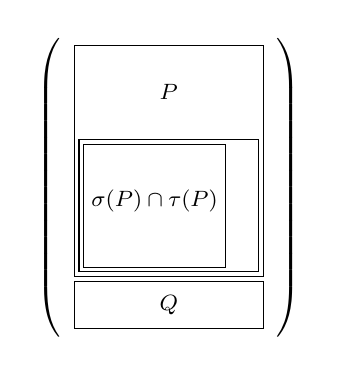
\begin{tikzpicture}[scale=0.6]
            \draw (-2,-1.9) rectangle (2,3);      % A
            \draw (-2,-3) rectangle (2,-2);     % B
            \draw (-1.9, -1.8) rectangle (1.9,1); % C
            \draw (-1.8, -1.7) rectangle (1.2, 0.9); % D
            \node at (0,2){\footnotesize$P$};
            \node at (0,-2.5) {\footnotesize$Q$};
            \node at (-0.3,-0.3){\footnotesize$\sigma(P) \cap \tau(P)$};
            \node at (-2.5,0){\(\left(\rule{0cm}{2.0cm}\right.\)};
            \node at (2.5,0){\(\left.\rule{0cm}{2.0cm}\right)\)};
        \end{tikzpicture}
        \caption{\label{fig:blocks}Separation of $M$ into blocks $P$ and $Q$, where the rows of $M$ are reordered for ease of presentation. 
            The Block on the left hand side shows the rows $\sigma(P) \cap \tau(P)$ within columns $I$ (moved to the left).}
        \end{center}
    \end{figure}


\begin{figure}
    \begin{center}
    \begin{tikzpicture}[scale=0.7]
        \draw (-2,-2) rectangle (2,3);      % A
        \draw (-2,-3) rectangle (9,-2);     % B
        \draw[dashed] (2,3) -- (9,-2);
        \draw[dashed] (9,-2) -- (18,-3);
         \draw[pattern=north east lines] (-2,-3.5) rectangle (18,-3); % Bottom area
        \node at (0,0){$R_A = (1-\epsilon)\tau(G)$};
        \node at (4,-2.5) {$R_B = (\epsilon - \epsilon^2)\tau(G)$};
        \node at (-2.5,0){\(\left(\rule{0cm}{2.4cm}\right.\)};
        \node at (19,0){\(\left.\rule{0cm}{2.4cm}\right)\)};

    \end{tikzpicture}
    \caption{\label{fig:section 2.1} Row sets on an instance $G$ . The bottom stripe depicts a block $R_C$ of $G$. All the blocks have binary values without wildcards.}
    \end{center}
\end{figure}


\begin{figure}
    \begin{center}
    \begin{tikzpicture}[scale=0.7]
        \draw (-2,-2) rectangle (2,3);      % A
        \draw (-2,-3) rectangle (9,-2);     % B
        \draw[dashed] (2,3) -- (9,-2);
        \draw (-2,-3.5) rectangle (18,-3);
        \draw[dashed] (9,-2) -- (18,-3);
        \draw (-2,-3.7) rectangle (18,-3);
         \draw[pattern=north east lines] (2,-3.7) rectangle (18,-3.5); % Bottom area
        \node at (0,0){$A_0$};
        \node at (5.5,-2.5) {$A_1$};
        \node at (9,-3.3) {$B_1$};
        \node at (-2.5,0){\(\left(\rule{0cm}{2.4cm}\right.\)};
        \node at (19,0){\(\left.\rule{0cm}{2.4cm}\right)\)};
        \draw (2,-3.7) to (2,-2);
        \draw (9,-3) to (9,-3);
    \end{tikzpicture}
    \caption{\label{fig:DP-analysis} Blocks $A_i, B_i$ on an instance $G$ for the $i^{th}$ iteration of DP in Lemma~\ref{lem:simpleDP}. The bottom stripe depicts a block $C_1$ of $G$.}
    \end{center}
\end{figure}

\begin{figure}
    \begin{center}
    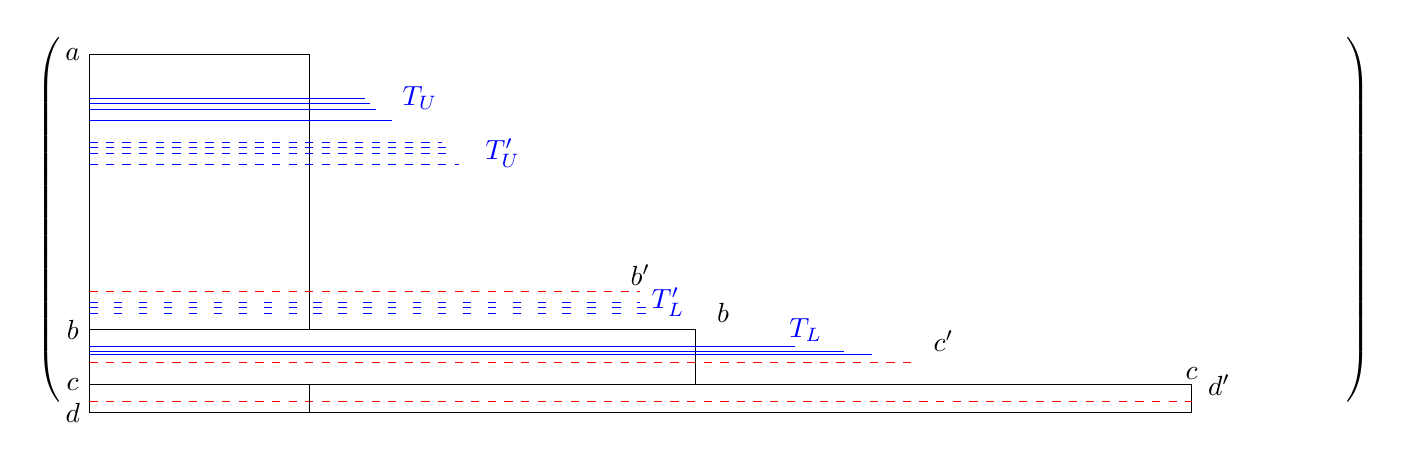
\begin{tikzpicture}[scale=0.7]
        \draw (-2,-2) rectangle (2,3);      % A
        \node at (-2.3,3) {$a$};
        \draw (-2,-3) rectangle (9,-2);     % B
%         \draw[dashed] (2,3) -- (9,-2);
%          \draw[dashed] (9,-2) -- (18,-3);
        \node at (-2.3,-2) {$b$};
        \node at (-2.3,-3) {$c$};
        \node at (-2.3,-3.5) {$d$};
        \draw[red,dashed] (-2,-1.3) -- (8,-1.3);
        \node at (8, -1) {$b'$};
        \node at (9.5, -1.7) {$b$};
        \node at (13.5, -2.2) {$c'$};
        \draw (-2,-3.5) rectangle (18,-3);
       \draw[red,dashed] (-2,-2.6) -- (13,-2.6);
        \draw[red,dashed] (-2,-3.3) -- (18,-3.3);
        \node at (18.5, -3) {$d'$};
        \node at (18, -2.8) {$c$};
%         \node[red] at (18.5, -3) {$B'_2$};
%          \draw (2,-3.7) rectangle (20,-3.5); % Bottom area
%         \node at (0,0){$A_0$};
%         \node at (0,-2.7) {$B_0$};
%         \node at (5.5,-1) {$B_0', T_U = T'_L$};
% 	\node[red] at (5.5,-1) {$B_0'$};
%        \node at (0,-3.3) {$B_1$};
%         \node[red] at (7,-2.8) {$B'_1$};
        \node at (-2.7,0){\(\left(\rule{0cm}{2.4cm}\right.\)};
        \node at (21,0){\(\left.\rule{0cm}{2.4cm}\right)\)};
         \draw (2,-3) to (2,-3.5);
%          \draw (9,-3.5) to (9,-3.7);
%          \node at (20.5,-3.6) {$B_2$};
         \draw[blue,dashed] (-2,1) -- (4.7,1);
         \draw[blue,dashed] (-2,1.2) -- (4.6,1.2);
         \draw[blue,dashed] (-2,1.3) -- (4.5,1.3);
         \draw[blue,dashed] (-2,1.4) -- (4.4,1.4);
         \node[blue,dashed] at (5.5, 1.2) {$T'_U$};

         \draw[blue] (-2,1.8) -- (3.5,1.8);
         \draw[blue] (-2,2) -- (3.2,2);
         \draw[blue] (-2,2.1) -- (3.1,2.1);
         \draw[blue] (-2,2.2) -- (3,2.2);
         \node[blue] at (4, 2.2) {$T_U$};
         
         \draw[blue] (-2,-2.3) -- (10.8,-2.3);
         \draw[blue] (-2,-2.4) -- (11.7,-2.4);
         \draw[blue] (-2,-2.45) -- (12.2,-2.45);
         \node[blue] at (11, -2) {$T_L$};
         
	\draw[blue,loosely dashed] (-2,-1.5) -- (8,-1.5);
	\draw[blue,loosely dashed] (-2,-1.6) -- (8.1,-1.6);
	\draw[blue, loosely dashed] (-2,-1.7) -- (8.1,-1.7);
         \node[blue] at (8.5, -1.5) {$T'_L$};
         

%         \draw (9,-3) to (9,-3);
    \end{tikzpicture}
    \caption{\label{fig:DP-crux1} Example of a child cell in the DP for the second string. The cell starting at $b'$ (drawn in red) is a child of the cell staring at $a$ (drawn in blue), because $b' > b$ and $T_U \cup T_L$ is disjoint from  $T'_U \cup T'_L$.}
    \end{center}
\end{figure}


\begin{figure}
    \begin{center}
    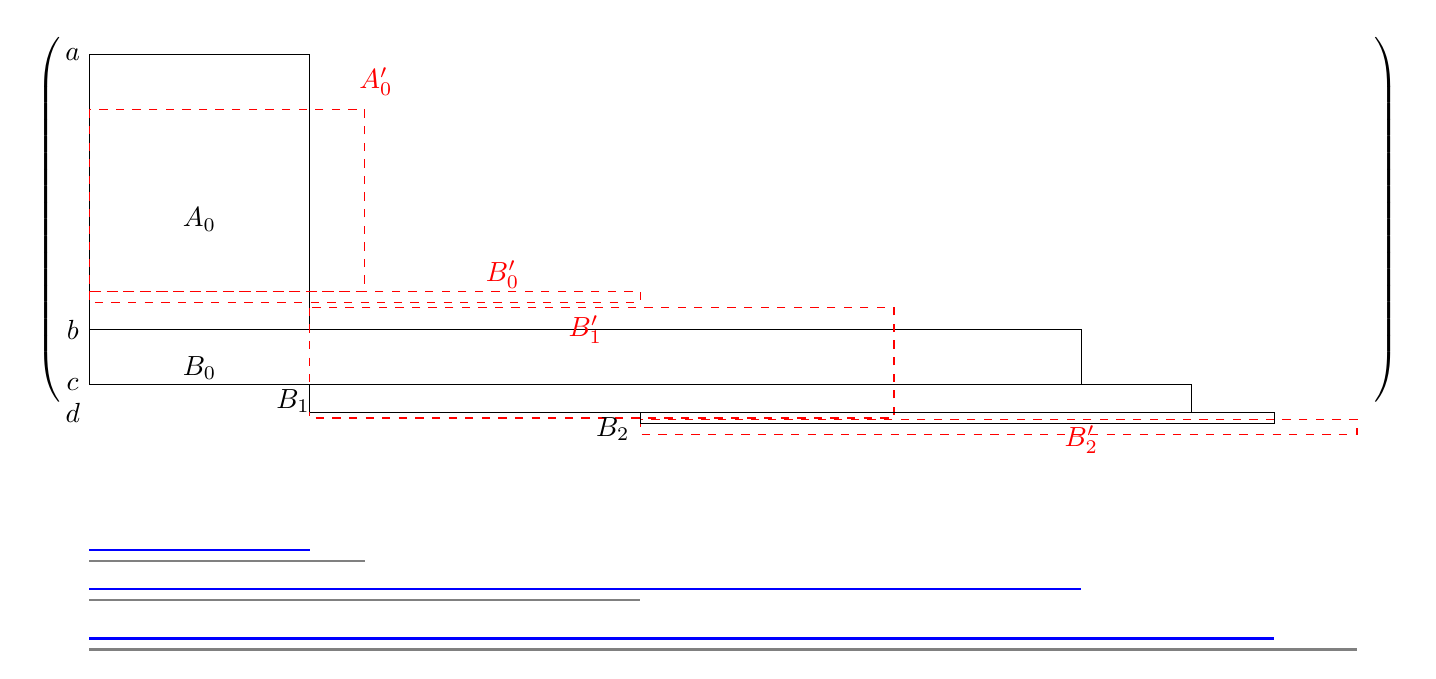
\begin{tikzpicture}[scale=0.7]
        \draw (-2,-2) rectangle (2,3);      % A
        \draw[red, dashed] (-2,2) rectangle (3,-1.3);
       
        \node at (-2.3,3) {$a$};
        \draw (-2,-3) rectangle (16,-2);     % B
%         \draw[dashed] (2,3) -- (9,-2);
%          \draw[dashed] (9,-2) -- (18,-3);
        \node at (-2.3,-2) {$b$};
        \node at (-2.3,-3) {$c$};
        \node at (-2.3,-3.5) {$d$};
        \draw[red,dashed] (-2,-1.3) rectangle (8,-1.5);
%         \node at (9, -1.3) {$a' \leftarrow b'$};
%         \node at (9.5, -1.8) {$a \leftarrow b$};
%         \node at (13.5, -1.5) {$b' \leftarrow c'$};
        \draw (2,-3.5) rectangle (18,-3);
       \draw[red,dashed] (2,-1.6) rectangle (12.6,-3.6);
         \draw[red,dashed] (8,-3.62) rectangle (21,-3.9);
%         \node at (20, -3) {$c'\leftarrow d'$};
%         \node at (18.5, -2.7) {$b\leftarrow c$};
         \node[red] at (16, -4) {$B'_2$};
         \draw (8,-3.7) rectangle (19.5,-3.5); % Bottom area
        \node at (0,0){$A_0$};
        \node[red] at (3.2,2.5){$A'_0$};
        \node at (0,-2.7) {$B_0$};
%         \node at (5.5,-1) {$B_0', T_U = T'_L$};
	\node[red] at (5.5,-1) {$B_0'$};
       \node at (1.7,-3.3) {$B_1$};
        \node[red] at (7,-2) {$B'_1$};
        \node at (-2.7,0){\(\left(\rule{0cm}{2.4cm}\right.\)};
        \node at (21.5,0){\(\left.\rule{0cm}{2.4cm}\right)\)};
         \draw (2,-3) to (2,-3.5);
%          \draw (9,-3.5) to (9,-3.7);
%          \node at (18.5, -2.7) {$b \leftarrow c$};
          \node at (7.5,-3.8) {$B_2$};
%           \node at (20.8,-3.4) {$c \leftarrow d$};
%         \draw (9,-3) to (9,-3);
% 	  \node at (0,-2) ${\sigma}$;
	 \draw[blue, thick] (-2,-6) -- (2,-6);
	 \draw[gray, thick] (-2,-6.2) -- (3,-6.2);
	 \draw[blue, thick] (-2,-6.7) -- (16,-6.7);
	 \draw[gray, thick] (-2,-6.9) -- (8,-6.9);
	 \draw[blue, thick] (-2,-7.6) -- (19.5,-7.6);
	 \draw[gray, thick] (-2,-7.8) -- (21,-7.8);
    \end{tikzpicture}
    \caption{\label{fig:DP-crux2} Blocks of an instance $M$ in the DP for the second string. 
        $B'_0$ is a child of $A_0$, $B'_1$ is a child of $A_0$, $B'_1$ is a child of $A_0$. The blue and gray lines represents $\sigma$ and $\sigma'$ respectively from first two iterations of DP. The sketch shows the switch example in the second iteration. }
    \end{center}
\end{figure}


% \begin{figure}
%     \begin{center}
%     \begin{tikzpicture}[scale=0.7]
%         \draw (-2,-2) rectangle (2,3);      % A
%         \node at (-2.3,3) {$a$};
%         \draw (-2,-3) rectangle (9,-2);     % B
%         \draw[dashed] (2,3) -- (9,-2);
%          \draw[dashed] (9,-2) -- (18,-3);
%         \node at (-2.3,-2) {$b$};
%         \node at (-2.3,-3) {$c$};
%         \node at (-2.3,-3.5) {$d$};
%         \draw[red,dashed] (-2,-1.3) rectangle (8,-2.37);
%         \node at (9, -1.3) {$a \leftarrow b'$};
%         \node at (9.5, -1.7) {$a'\leftarrow b$};
%         \node at (13.5, -2.2) {$b \leftarrow c'$};
%         \draw (-2,-3.5) rectangle (18,-3);
%        \draw[red,dashed] (2,-2.5) rectangle (12.6,-3.25);
%         \draw[red,dashed] (9,-3.3) rectangle (19,-3.6);
%         \node at (20, -3) {$c' \leftarrow d'$};
%         \node at (18.5, -2.7) {$b'\leftarrow c$};
%         \node[red] at (16, -4) {$B'_2$};
%          \draw (2,-3.7) rectangle (20,-3.5); % Bottom area
%         \node at (0,0){$A_0$};
%         \node at (0,-2.5) {$B'_0$};
% %         \node at (5.5,-1) {$B_0', T_U = T'_L$};
% 	\node[red] at (5.5,-1) {$B_0$};
%        \node at (0,-3.3) {$B'_1$};
%         \node[red] at (7,-2.8) {$B_1$};
%         \node at (-2.7,0){\(\left(\rule{0cm}{2.4cm}\right.\)};
%         \node at (21,0){\(\left.\rule{0cm}{2.4cm}\right)\)};
%          \draw (2,-3) to (2,-3.5);
%          \draw (9,-3.5) to (9,-3.7);
% %          \node at (18.5, -2.7) {$b=c$};
%          \node at (20,-4) {$B_2$};
%           \node at (20.8,-3.4) {$c \leftarrow d$};
% %         \draw (9,-3) to (9,-3);
%     \end{tikzpicture}
%     \caption{\label{fig:DP-crux3} This sketch shows the different cases of the previous example. 
%         The only difference is that the predecessors come from the other solution string. 
%         Again assuming that the disjointness property always holds,  the $\zeta$ cell is a child of the $\zeta'$ cell because $c' < c$. 
%         The predecessors do not have the child relationship, because $b > b'$ implies that the rows from $B'_1$ and $B'_2$ can interfere with each other and the rows $B_1$ and $B'_0$ interfere.}
%     \end{center}
% \end{figure}
% 
% \begin{figure}
%     \begin{center}
%     \begin{tikzpicture}[scale=0.7]
%         \draw (-2,-2) rectangle (2,3);      % A
%         \node at (-2.3,3) {$a$};
%         \draw (-2,-3) rectangle (9,-2);     % B
%         \draw[dashed] (2,3) -- (9,-2);
%          \draw[dashed] (9,-2) -- (18,-3);
%         \node at (-2.3,-2) {$b$};
%         \node at (-2.3,-3) {$c$};
%         \node at (-2.3,-3.5) {$d$};
%         \draw[dashed, thick, blue] (-2,-1.3) rectangle (8,-3.45);
% %         \draw[pattern=north east lines] (-2,-3.3) rectangle (19,-3.5);
%         \node at (9, -1.3) {$a' = b'$};
%         \node at (9.5, -1.7) {$a = b$};
%         \node at (13.5, -2.2) {$b' = c'$};
%         \draw (-2,-3.5) rectangle (18,-3);
%        \draw[red,dashed] (2,-2.5) rectangle (12.6,-3.4);
%          \draw[red, dashed] (9,-3.3) rectangle (19,-3.6);
%         \node at (20, -3) {$c' = d'$};
%         \node[red] at (18.5, -3) {$B'_2$};
%          \draw (2,-3.7) rectangle (20,-3.5); % Bottom area
%         \node at (0,0){$A_0$};
%         \node at (0,-2.5) {$B_0$};
%          \node at (0,-3.3) {$B_1$};
% %         \node at (5.5,-1) {$B_0', T_U = T'_L$};
% 	\node[blue] at (5.5,-1) {$B_0'$};
%         \node[red] at (7,-2.8) {$B'_1$};
%         \node at (-2.7,0){\(\left(\rule{0cm}{2.4cm}\right.\)};
%         \node at (21,0){\(\left.\rule{0cm}{2.4cm}\right)\)};
%          \draw (2,-3) to (2,-3.5);
%          \draw (9,-3.5) to (9,-3.7);
%          \node at (20.5,-3.6) {$B_2$};
% %         \draw (9,-3) to (9,-3);
%     \end{tikzpicture}
%     \caption{\label{fig:DP-crux4} this figure is wrong?????, Blocks on an instance $G$ in DP, when predecessors are both parent and children because rows from block $B_0'$, $B'_1$ and $B_2'$ interfere with each other.}
%     \end{center}
% \end{figure}

\begin{figure}
    \begin{center}
    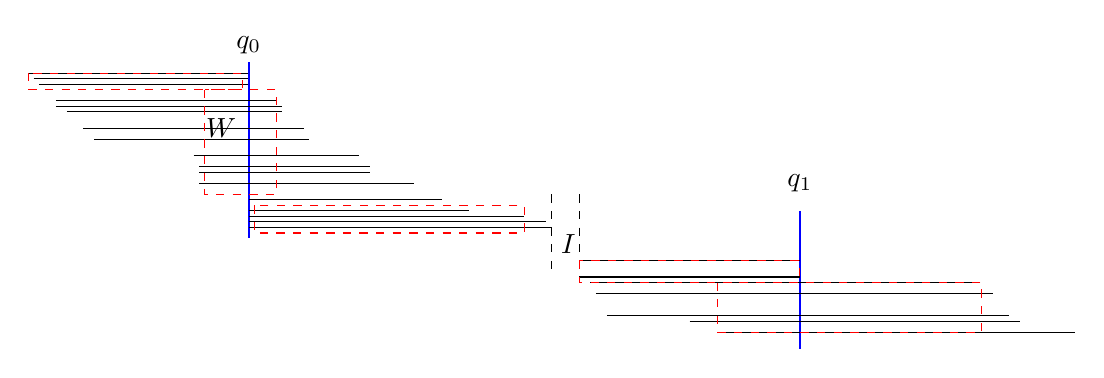
\begin{tikzpicture}[scale=0.7]
	\draw (0,0) -- (4,0);
	\draw (0.1,-.1) -- (4,-.1);
	\draw (0.2,-.2) -- (4,-.2);
	\draw[blue,thick] (4,.2) -- (4,-3);
	\node at (4,.5) {$q_0$};
	\node at (3.5,-1) {$W$};
	\draw (0.5,-.5) -- (4.5,-0.5);
	\draw (0.5,-.6) -- (4.6,-0.6);
	\draw (0.7,-.7) -- (4.6,-0.7);
	\draw (1,-1) -- (5,-1);
	\draw (1.2,-1.2) -- (5.1,-1.2);
	\draw (3,-1.5) -- (6,-1.5);
	\draw (3.1,-1.7) -- (6.2,-1.7);
	\draw (3.1,-1.8) -- (6.2,-1.8);
	\draw (3.1,-2) -- (7,-2);
	\draw (4,-2.3) -- (7.5,-2.3);
	\draw (4,-2.5) -- (8,-2.5);
	\draw (4,-2.6) -- (9,-2.6);
	\draw (4,-2.7) -- (9.4,-2.7);
	\draw (4,-2.8) -- (9.5,-2.8);
	\draw[blue,thick] (14,-2.5) -- (14,-5);
	\node at (14, -2) {$q_1$};
% 	\draw (5,-3.1) -- (11,-3.1);
% 	\draw (5.1,-3.2) -- (11.1,-3.2);
% 	\draw (5.2,-3.3) -- (11.2,-3.3);
	\draw (10,-3.4) -- (14,-3.4);
	\draw[dashed] (9.5,-2.2) to (9.5,-3.6);
	\draw[dashed] (10,-2.2) to (10,-3.6);
	\draw (10,-3.7) -- (14,-3.7);
	\draw (10.2,-3.8) -- (17.2,-3.8);
	\draw (10.3,-4) -- (17.5,-4);
	\draw (10.5,-4.4) -- (17.8,-4.4);
	\draw (12,-4.5) -- (18,-4.5);
	\draw (12.5,-4.7) -- (19,-4.7);
	\node at (9.8,-3.1) {$I$};
 	\draw[red, dashed] (0,0) rectangle (3.89,-.3);
  	\draw[red, dashed] (3.2,-.3) rectangle (4.5,-2.2);
  	\draw[red, dashed] (10,-3.4) rectangle (14,-3.8);
  	\draw[red, dashed] (12.5,-3.8) rectangle (17.3,-4.7);
  	\draw[red, dashed] (4.1,-2.4) rectangle (9,-2.9);
    \end{tikzpicture}
    \caption{\label{fig:second_instance1} Blocks represented by ranges shown in red on an instance $M$ and the blue lines are the columns, $I$ and $C$ shows the empty interval and central region respectively.}
    \end{center}
\end{figure}

\begin{figure}
    \begin{center}
    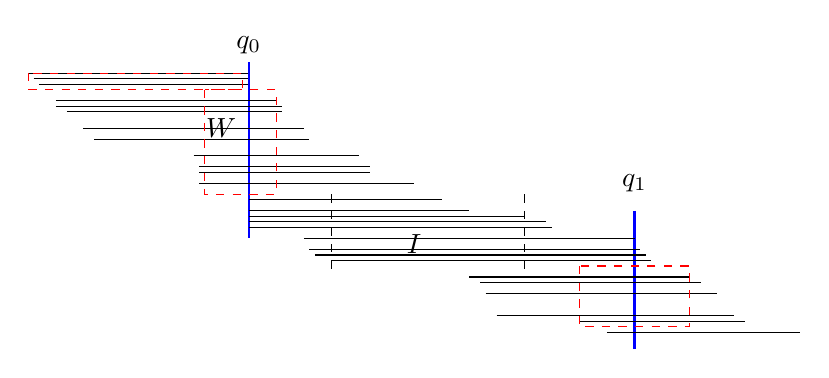
\begin{tikzpicture}[scale=0.7]
	\draw (0,0) -- (4,0);
	\draw (0.1,-.1) -- (4,-.1);
	\draw (0.2,-.2) -- (4,-.2);
	\draw[blue,thick] (4,.2) -- (4,-3);
	\node at (4,.5) {$q_0$};
	\node at (3.5,-1) {$W$};
	\draw (0.5,-.5) -- (4.5,-0.5);
	\draw (0.5,-.6) -- (4.6,-0.6);
	\draw (0.7,-.7) -- (4.6,-0.7);
	\draw (1,-1) -- (5,-1);
	\draw (1.2,-1.2) -- (5.1,-1.2);
	\draw (3,-1.5) -- (6,-1.5);
	\draw (3.1,-1.7) -- (6.2,-1.7);
	\draw (3.1,-1.8) -- (6.2,-1.8);
	\draw (3.1,-2) -- (7,-2);
	\draw (4,-2.3) -- (7.5,-2.3);
	\draw (4,-2.5) -- (8,-2.5);
	\draw (4,-2.6) -- (9,-2.6);
	\draw (4,-2.7) -- (9.4,-2.7);
	\draw (4,-2.8) -- (9.5,-2.8);
	\draw[blue,thick] (11,-2.5) -- (11,-5);
	\node at (11, -2) {$q_1$};
	\draw (5,-3) -- (11,-3);
	\draw (5.1,-3.2) -- (11.1,-3.2);
	\draw (5.2,-3.3) -- (11.2,-3.3);
	\draw (5.5,-3.4) -- (11.3,-3.4);
	\draw[dashed] (5.5,-2.2) to (5.5,-3.6);
	\draw[dashed] (9,-2.2) to (9,-3.6);
	\draw (8,-3.7) -- (12,-3.7);
	\draw (8.2,-3.8) -- (12.2,-3.8);
	\draw (8.3,-4) -- (12.5,-4);
	\draw (8.5,-4.4) -- (12.8,-4.4);
	\draw (10,-4.5) -- (13,-4.5);
	\draw (10.5,-4.7) -- (14,-4.7);
	\node at (7,-3.1) {$I$};
 	\draw[red, dashed] (0,0) rectangle (3.89,-.3);
  	\draw[red, dashed] (3.2,-.3) rectangle (4.5,-2.2);
  	\draw[red, dashed] (10,-3.5) rectangle (12,-4.6);
%   	\draw[red, dashed] (4.1,-2.4) rectangle (9,-2.9);
    \end{tikzpicture}
    \caption{\label{fig:second_instance2} This sketch shows non-dominance example in region $I$.}
    \end{center}
\end{figure}

% \begin{figure}
%     \begin{center}
%     \begin{tikzpicture}[scale=0.7]
% 	\draw (0,0) -- (4,0);
% 	\draw (0.1,-.1) -- (4,-.1);
% 	\draw (0.2,-.2) -- (4,-.2);
% 	\draw[blue,thick] (4,.2) -- (4,-3);
% 	\node at (4,.5) {$q_0$};
% 	\node at (3.5,-1) {$C$};
% 	\draw (0.5,-.5) -- (4.5,-0.5);
% 	\draw (0.5,-.6) -- (4.6,-0.6);
% 	\draw (0.7,-.7) -- (4.6,-0.7);
% 	\draw (1,-1) -- (5,-1);
% 	\draw (1.2,-1.2) -- (5.1,-1.2);
% 	\draw (3,-1.5) -- (6,-1.5);
% 	\draw (3.1,-1.7) -- (6.2,-1.7);
% 	\draw (3.1,-1.8) -- (6.2,-1.8);
% 	\draw (3.1,-2) -- (7,-2);
% 	\draw (4,-2.3) -- (7.5,-2.3);
% 	\draw (4,-2.5) -- (8,-2.5);
% 	\draw (4,-2.6) -- (9,-2.6);
% 	\draw (4,-2.7) -- (9.4,-2.7);
% 	\draw (4,-2.8) -- (9.5,-2.8);
% 	\draw[blue,thick] (11,-2.5) -- (11,-5);
% 	\node at (11, -2) {$q_1$};
% % 	\draw (5,-3) -- (11,-3);
% % 	\draw (5.1,-3.2) -- (11.1,-3.2);
% % 	\draw (5.2,-3.3) -- (11.2,-3.3);
% 	\draw (8,-3.4) -- (11,-3.4);
% 	\draw[dashed] (5.5,-2.2) to (5.5,-3.6);
% 	\draw[dashed] (9.5,-2.2) to (9.5,-3.6);
% % 	\draw (8,-3.7) -- (12,-3.7);
% 	\draw (10,-3.8) -- (12.2,-3.8);
% 	\draw (10.3,-4) -- (12.5,-4);
% 	\draw (10.3,-4.4) -- (12.8,-4.4);
% % 	\draw (10,-4.5) -- (13,-4.5);
% 	\draw (10.3,-4.6) -- (14,-4.6);
% 	\draw (10.3,-4.5) -- (14,-4.5);
% 	\draw (10.3,-4.8) -- (14,-4.8);
% 	\node at (7,-3.1) {$I$};
%  	\draw[red, dashed] (0,0) rectangle (3.89,-.3);
%   	\draw[red, dashed] (3.2,-.3) rectangle (4.5,-2.2);
%   	\draw[red, dashed] (10.3,-3.5) rectangle (12,-4.8);
% %   	\draw[red, dashed] (4.1,-2.4) rectangle (9,-2.9);
%     \end{tikzpicture}
%     \caption{\label{fig:second_instance3} This sketch shows dominance example in $I$.}
%     \end{center}
% \end{figure}



\begin{figure}
    \begin{center}
    \begin{tikzpicture}[shorten >=1pt,node distance=2cm,on grid,auto, scale =.5]
    \begin{scope}
     \draw[blue,thick] (10,.2) -- (10,-6);
     \draw (5,-0.5) -- (15,-0.5);
     \draw (7,-1) -- (13,-1);
     \draw (8,-1.5) -- (11,-1.5);
     \draw (9,-2) -- (11,-2);
     \draw (9,-2.5) -- (15,-2.5);
     \draw (7.5,-3) -- (13,-3);
     \draw (6,-3.5) -- (10.5,-3.5);
     \draw (5,-4) -- (10.5,-4);
     \node at (8,.2) {$\overleftarrow{A}$};
     \node at (10,.5) {$c$};
      \node at (12,.2) {$\overrightarrow{A}$};
      \node at (10,-6.8) {(a)};
     \end{scope}
     \begin{scope}[xshift=15cm]
      
     \draw[blue,thick] (7,.2) -- (7,-6);
     \draw[blue,thick] (13,.2) -- (13,-6);
     \draw[blue,thick] (19,.2) -- (19,-6);
     \draw[blue,thick,dashed] (10,.2) -- (10,-6);
     \draw[blue,thick,dashed] (16,.2) -- (16,-6);
     \node at (2.5,-1.5) {$L_1$};
     \node at (7,0.5) {$q_{1,0}$};
     \node at (10,0.5) {$q_{1,1}$};
     \node at (13,0.5) {$q_{1,2}$};
     \node at (16,0.5) {$q_{1,3}$};
     \node at (19,0.5) {$q_{1,4}$};
     \draw (1,-0.5) -- (7,-0.5);
     \draw (3,-0.7) -- (8,-0.7);
     \draw (5,-0.9) -- (8,-0.9);
     \draw (6,-1.2) -- (11,-1.2);
     \draw (7,-1.5) -- (13,-1.5);
     \draw (8,-1.7) -- (11,-1.7);
     \draw (9,-1.9) -- (12,-1.9);
     \draw (9,-2.1) -- (13,-2.1);
     \draw (9,-2.3) -- (14,-2.3);
     \draw (8,-2.5) -- (12,-2.5);
     \draw (9.5,-2.9) -- (14,-2.9);
     \draw (11,-2.7) -- (16,-2.7);
     \draw (13,-3.1) -- (19,-3.1);
     \draw (14,-3.3) -- (19,-3.3);
     \draw (17,-3.5) -- (21,-3.5);
      \draw (15,-3.7) -- (21,-3.7);
      \node at (13,-6.8) {(b)};
     \end{scope}

     
    \end{tikzpicture}
    \caption{\label{fig:gen_instance1} (a) Sub-matrices for rooted \GMEC. (b) For a single-length-class instance, the sketch shows the strings crossing each column either exactly once or exactly twice.}
    \end{center}
\end{figure}

\begin{figure}
    \begin{center}
    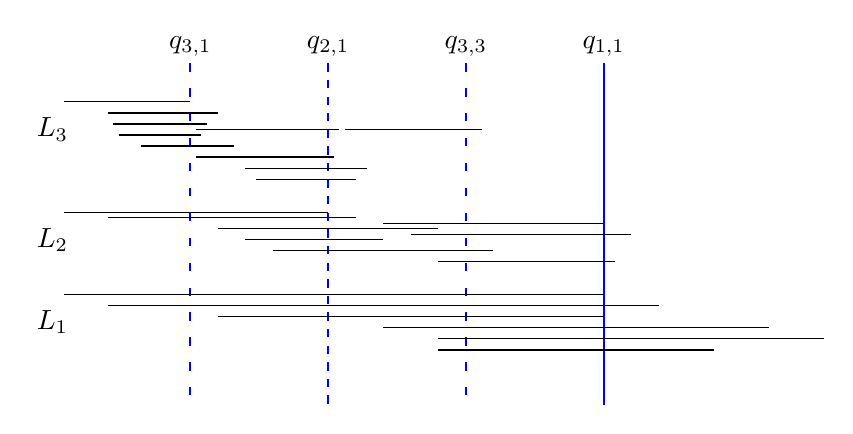
\begin{tikzpicture}[scale=0.7]
	\node at (2.5, .5) {$q_{3,1}$};
	\node at (5, .5) {$q_{2,1}$};
	\node at (7.5, .5) {$q_{3,3}$};
	\node at (10, .5) {$q_{1,1}$};
% 	\draw[blue,thick] (0,.2) -- (0,-6);
	\draw[blue,thick] (10,.2) -- (10,-6);
	\draw[blue,thick, dashed] (5,.2) -- (5,-6);
	\draw[blue,thick, loosely dashed] (2.5,.2) -- (2.5,-6);
	\draw[blue,thick, loosely dashed] (7.5,.2) -- (7.5,-6);
	\draw (.2,-4) -- (10,-4);
	\draw (1,-4.2) -- (11,-4.2);
	\draw (3,-4.4) -- (10,-4.4);
	\draw (6,-4.6) -- (13,-4.6);
	\draw (7,-4.8) -- (14,-4.8);
	\draw (7,-5) -- (12,-5);
	\node at (0,-4.5) {$L_1$};

	\draw (.2,-2.5) -- (5,-2.5);
	\draw (1,-2.6) -- (5.5,-2.6);
	\draw (3,-2.8) -- (7,-2.8);
	\draw (3.5,-3.0) -- (6,-3.0);
	\draw (4,-3.2) -- (8,-3.2);
	\node at (0,-3) {$L_2$};

	
	\draw (6,-2.7) -- (10,-2.7);
	\draw (6.5,-2.9) -- (10.5,-2.9);
	\draw (7,-3.4) -- (10.2,-3.4);
	
	\draw (.2,-0.5) -- (2.5,-0.5);
	\draw (1,-0.7) -- (3,-0.7);
	\draw (1.1,-0.9) -- (2.8,-0.9);
	\draw (1.2,-1.1) -- (2.7,-1.1);
	\draw (1.6,-1.3) -- (3.3,-1.3);
	
	\draw (2.6,-1.5) -- (5.1,-1.5);
	\draw (3.5,-1.7) -- (5.7,-1.7);
	\draw (3.7,-1.9) -- (5.5,-1.9);
	\draw (2.6,-1.0) -- (5.2,-1.0);
	\draw (5.3,-1.0) -- (7.8,-1.0);
	\node at (0,-1) {$L_3$};
    \end{tikzpicture}
    \caption{\label{fig:gen_instance2} Different length classes $L_1$ with corresponding column $q_{1,1}$, 
        $L_2$ with corresponding columns $q_{2,1}, q_{2,2} = q_{1,1}$, 
        and $L_3$ with corresponding columns $q_{3,1}, q_{3,2} = q_{2,1}, q_{3,3}, q_{3,4} = q_{1,1}$.}
    \end{center}
\end{figure}




